\documentclass[conference]{IEEEtran}
\IEEEoverridecommandlockouts
\usepackage{cite}
\usepackage{amsmath,amssymb,amsfonts}
\usepackage{graphicx}
\graphicspath{{figures/}}
\usepackage{textcomp}
\usepackage{xcolor}
\usepackage{booktabs}
\usepackage{array}
\usepackage{url}
\usepackage{color}
\usepackage{soul}
\sethlcolor{yellow}
\usepackage{pgfplots}
\pgfplotsset{compat=1.18}      

% ---- TODO helper: remove \showtodos to hide all TODO notes before submission
\newcommand{\showtodos}{}
\ifdefined\showtodos
  \newcommand{\todo}[1]{\textcolor{red}{\textbf{[TODO: #1]}}}
\else
  \newcommand{\todo}[1]{}
\fi

\begin{document}

\title{Psycholinguistic Style in Library Documentation Across Ecosystems and Authorship}

\author{
\IEEEauthorblockN{Max Shi}
\IEEEauthorblockA{
\textit{Computer Science and Software Engineering}\\
\textit{University of Canterbury}\\
Christchurch, New Zealand\\
msh254@uclive.ac.nz}
\and
\IEEEauthorblockN{Supervisor: Mathieu Nassif}
\IEEEauthorblockA{
\textit{Computer Science and Software Engineering}\\
\textit{University of Canterbury}\\
Christchurch, New Zealand\\
mathieu.nassif@canterbury.ac.nz}
}

\maketitle
\thispagestyle{plain}
\pagestyle{plain}

\begin{abstract}
Documentation style may vary across software ecosystem and also between human and generated text. However, to truly see the differences between these, an empirical measurement and analysis must be completed. Understanding these differences can inform documentation guidance and may help evaluate generated documentation. This study uses Linguistic Inquiry and Word Count (LIWC-22), to compare Java and Python library documentation across 15 dimensions, selected in a pilot and fixed before a confirmatory collection. Additionally, a paired corpus will compare human written READMEs with documentation generated from two LLM models for 50 libraries per ecosystem. Analysis will combine statistical tests, effect sizes and construct validity audits and classifications. Overall, no ecosystem difference met the full decision rule after checks and corrections, and on average 98.8\% of measured variance lay within ecosystems. Ecosystem classification detected a signal, with a macro-F1 of 0.672, but this was also below the required 0.75. Generated documentation consistently contained a higher share of long words. Therefore, a word-length threshold was able to distinguish human and generated documents with a macro-F1 of 0.810, with 94\% sensitivity and 67\% specificity. Audits also identified several problems pertaining to dictionary-interpretation, unequal preprocessing and mismatched document scope. The results support word length as a signal, under these evaluated generation conditions, while also showing the importance of corpus validation, and the limitations of interpreting linguistic scores as ecosystem or authorship characteristics.
\end{abstract}

\section{Introduction}
\label{sec:intro}

Software documentation is the primary connection between a technology and the end users. The quality of this documentation depends on a few factors: the technical accuracy of the content, and also how the information has been conveyed. Word use and choice can provide measurable signals of psychological processes \cite{tausczik2010}. However, whether or not these linguistic choices can affect the perceived authority or accessibility of the documentation requires further study.

Software ecosystems, like Python or Java, bring together different libraries, contributors and tools around a specific language. Thus, small differences in conventions and expectations may produce distinct linguistic patterns, as register can vary given these situation contexts \cite{biber1988}. By comparing these patterns, this can establish whether developers moving between ecosystems may also encounter different documentation styles. Additionally, LLMs can answer programming questions ~\cite{kabir2024}, which raises a seperate questions: does generated library documentation reproduce this ecosystem variation or flatten it?

These questions require measurements which can be interpreted in technical text. Linguistic Inquiry and Word Count (LIWC) measures linguistic features of text using dictionary categories, and computed text statistics \cite{boyd2022}. Sajadi et al. Identifies evaluation gaps and concerns pertaining to technical vocabulary in software engineering applications of LIWC \cite{sajadi2026}. Technical documentation contains specialised vocabulary and identifies, confusing the true meaning of these dictionary categories. Therefore, when applying LIWC in a SE context, LIWC scores require checks that the affected dimensions do actually measure the intended constructs.

This report presents a quantitative study of documentation style across Java and Python libraries and between human and LLM-generated documentation. The dimension list and decision rule were fixed before the confirmatory data collection. The contributions of this report are: (i) no cross-ecosystem difference met the full decision rule at either confirmatory sample size even after the relevant validity checks and corrections, although classification detected an ecosystem signal, but below the specified reliability threshold; (ii) generated documentation contained a higher proportion of long words across both evaluated models and ecosystems, with lower dispersion in all nine significant construct-valid comparisons; and (iii) audits identified limitations in interpreting selected LIWC dimensions, unequal preprocessing and mismatched software scope in paired documents.

Section~\ref{sec:background} states the objectives, Section~\ref{sec:related} reviews related work, Section~\ref{sec:design} describes the study design, Sections~\ref{sec:results}--\ref{sec:results-method-findings} report the results, and Sections~\ref{sec:results-discussion}--\ref{sec:conclusion} discuss them and concludes.

\section{Background and Objectives}
\label{sec:background}

This individual project was conducted at the University of Canterbury under the supervision of Dr.~Mathieu Nassif and Dr.~Ben Adams, with no external collaborators, non-disclosure agreement or pre-existing results from earlier projects.  LIWC-22 was used through its licensed desktop interface. Generation costs limited the RQ3 paired corpus to 50 libraries per ecosystem (200 total).

The objective of this paper is to determine whether documentation style varies with ecosystem and authorship. The study addresses the following research questions:

\textbf{RQ1 --- Cross-ecosystem differences.} How do psycholinguistic patterns of
library documentation vary across different software ecosystems?

\textbf{RQ2 --- Within-ecosystem variance.} How consistent are documentation
styles within each ecosystem, and how does intra-ecosystem variation compare to
inter-ecosystem differences?

\textbf{RQ3 --- Human versus LLM-generated documentation.} How do the
psycholinguistic characteristics of AI-generated documentation differ from
human-written documentation for the same libraries?

\textbf{RQ4 --- Ecosystem fingerprinting.} To what extent do psycholinguistic
profiles alone serve as a reliable signal of ecosystem origin in library
documentation?

The questions are ordered by their analytical relationships. RQ2 examines whether domain composition could contribute to the differences assessed in RQ1; its domain tests do not establish the absence of confounding. RQ4 complements RQ1's per-dimension comparisons by testing whether combinations of features predict ecosystem origin.

\textbf{Success criteria and expected impact.} The success of this project is measured by whether each research question is answered with evidence, where the reliability and limitations can be evaluated, rather than if differences are detected. RQ1 and RQ3 use rank-based comparisons, with a decision rule requiring Holm-adjusted $p < 0.05$ and $|\delta| \ge 0.33$; construct-validity checks defines our interpretation (Section~\ref{sec:rule}). RQ2 separates within- and between-ecosystem variance and assesses functional-domain effects using $\eta^2_H$. RQ4 evaluates ecosystem prediction using macro-F1, with $0.75$ as the specified reliability criterion. Through these findings, they can inform whether documentation-style guidance requires ecosystem-specific evidence,  characterise differences between human and generated documentation, and can assess the usefulness and limitations of using linguistic features document origin prediction.

\section{Related Work}
\label{sec:related}

\subsection{Search Method}

Because a single keyword string cannot cover a project spanning several literatures, the search was organised into six rounds, each targeting a specific area: (1) LIWC applied to SE text, (2) documentation quality and style, (3) LLM-generated versus human text, (4) sentiment and emotion in developer communication, (5) register variation in corpus linguistics, and (6) community-level linguistic behaviour in open source. Round 1 was informed by Sajadi et al.'s search for LIWC applications in software engineering ~\cite{sajadi2026}, but the search in this paper uses different databases, search fields and eligibility criteria. Studies were included if they were peer-reviewed (or the LIWC manual), related to developer-produced or developer-facing text, and reported an empirical measurement. Texts were excluded if LIWC was used incidentially, or the text was not in English.

The primary search (May 2026, ten sources) retrieved approximately 1{,}400 records and, after de-duplication, screening and citation chaining, yielded 27 included works. A supplementary claim-driven searching and methodological background reading provided additional references. A separate Scopus verification search in September 2026 returned 1{,}624 unique records using the sixteen search strings. Further information may be found in the Appendix~\ref{annex:search}.

\subsection{Psycholinguistic Analysis of Software-Engineering Text}

LIWC maps words onto psychological and linguistic categories \cite{tausczik2010,boyd2022}. Dictionary revisions can change scores, so comparisons across releases depend on version and dimension being compared~\cite{pennebaker2015,boyd2022}. This motivates the single-version design used here. Sajadi et al. identify evaluation gaps and concerns about technical vocabulary in software-engineering applications
\cite{sajadi2026}.

Related work benchmarks sentiment tools~\cite{novielli2018}, develops and evaluates 'sentiment-polarity' detection~\cite{calefato2018}, characterises developer linguistic behaviour across social statuses in open-source projects~\cite{han2024}. These examples do not establish an absence of documentation research, but the question here concerns the selected linguistic features and comparisons across ecosystems and authorship conditions.

\subsection{Documentation as a Text Artefact}

Documentation research addresses learning, use, quality and content. Robillard and DeLine identify documentation and learning resources as major obstacles to API learning~\cite{robillard2011}; Uddin and Robillard describe content and presentation failures~\cite{uddin2015}. Meng et al. observe how developers use documentation~\cite{meng2019}, and Tang and Nadi evaluate documentation quality, including readability~\cite{tang2023}. Other studies classify README content~\cite{prana2019}, identify knowledge patterns in API reference documentation~\cite{maalej2013}, and analyse documentation issues including presentation and readability~\cite{aghajani2019}. These studies addresses several aspects of documentation, but this present study only focuses on the distribution of selected psycholinguistic features across ecosystems and authorship conditions.

\subsection{Generated Versus Human Text}

Kabir et al.~\cite{kabir2024} found incorrect information in 52\% of 517 sampled ChatGPT answers. But in a separate study with 12 programmers, participants preferred ChatGPT answers in 35\% of comparisons, citing
comprehensiveness and language style. This motivates examining generated documentation's style separately from its correctness. Sandler et al.~\cite{sandler2024} compare matched human and ChatGPT-generated
dialogues using LIWC categories, including differences in means and variances. Their work focuses on lingustic differences in conversational text, whereas this study examines library documentation. Within the studies retrieved and screened in the review, there was no identified study which paired human and LLM-generated documentation for comparison (from the same library).

\subsection{Register Variation and Positioning}

Prior work such as Biber's multi-dimensional analysis \cite{biber1988} established that written register may vary systematically across situational contexts, which is the foundation for the idea of treating an ecosystem as a register boundary, motivating the test for cross-ecosystem differences.

\section{Study Design}
\label{sec:design}

\subsection{Corpus and Extraction}

The study is implemented as a five-stage batch pipeline (Fig.~\ref{fig:pipeline}): frame construction from registry metadata, repository acquisition, prose extraction and normalisation, LIWC-22 scoring, and statistical analysis. RQ3 adds a branch which extracts each library's public API surface and generates documentation from it. Human and generated text pass through the same prose-extraction step prior to scoring. Intermediate files separate acquisition, extraction, manual LIWC scoring and analysis, allowing these stages to be repeated without rerunning the entire pipeline. The pipeline is written in Python, using pandas, SciPy and scikit-learn for analysis and Matplotlib for figures. Repositories are acquired with \texttt{git}, and generation uses the model providers' APIs.

\begin{figure}[t]
\centering
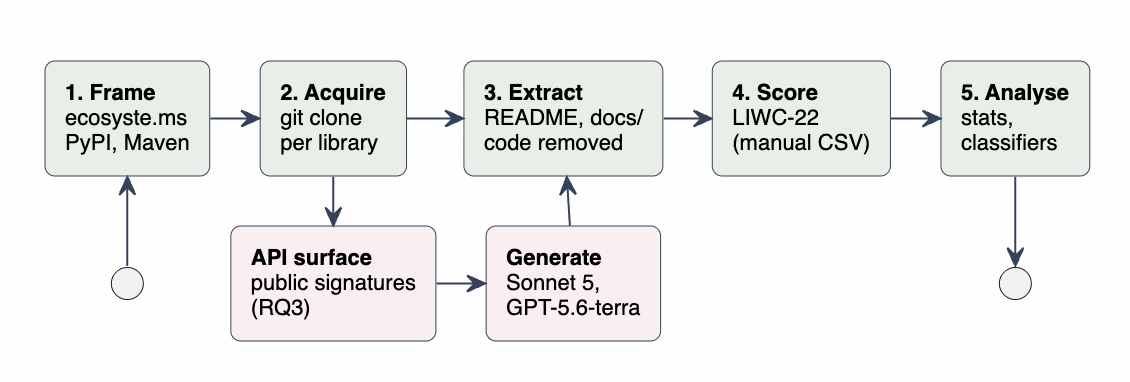
\includegraphics[width=0.85\columnwidth]{pipeline.png}
\caption{Study pipeline. Human documentation and API-based LLM output pass through shared prose extraction before LIWC-22 scoring. Ecosystem analyses use repository documentation; paired human--LLM analyses use READMEs.}
\label{fig:pipeline}
\end{figure}

\textbf{Design choices.} \emph{Instrument:} LIWC-22 was selected to measure multiple linguistic dimensions rather than sentiment alone, the focus of software-engineering sentiment tools~\cite{novielli2018,calefato2018}. LIWC categories support interpretation at a dimension-level, subject to the construct-validity audit in Section~\ref{sec:rule}. \emph{Documentation source:} repository-shipped documentation was used instead of hosted documentation sites, allowing for easier acquisition. \emph{Generation input:} models received public API signatures rather than the human README, avoiding direct access to the comparison text. Two models from different providers were used to assess model specificity. \emph{Classifiers:} RQ4 compares linear classifiers with a nonlinear random forest to assess whether predictive performance depends on the model family.

The population is published open-source library packages listed on PyPI or Maven Central with at least one released version and at least one human-readable documentation surface. ``Documentation'' throughout this report, denotes what a library ships in its repository: for RQ1 and RQ2, the README together with any \texttt{docs/}, \texttt{doc/} or \texttt{documentation/} tree, concatenated in a stable order (median 16-19 files per library); for RQ3 and RQ4 authorship, the README alone, so that a single human-authored README can be paired with a single generated one. Registry metadata comes from the ecosystem.ms Packages service, as it offered a direct API, and allowed for a more uniform schema across both registries. The
confirmatory frame (\texttt{frame\_20260712}) is $n=200$ libraries per ecosystem under a seeded sample; a second independent frame at $n=1000$ per ecosystem was also built later for a higher-power re-estimation. Prose extraction converts each source to plain text through a format-specific path and---importantly---\emph{removes
code}: \texttt{code}, \texttt{pre}, \texttt{script} and related elements are decomposed before extraction, for reasons given in Section~\ref{sec:results-method-findings}.

\subsection{LIWC and the Fifteen Dimensions}

LIWC-22~\cite{boyd2022} scores a text by matching each word against a set of dictionary categories, or \emph{dimensions}, and reporting the percentage of the text's words that fall into each. However, a few dimensions are computed rather than looked up: \texttt{WPS} is the mean number of words per sentence, \texttt{BigWords} the percentage of words of seven or more letters, and \texttt{Tone} a composite dimension where a higher value indicate more positive tone.

A pilot screened 59 LIWC dimensions; 15 were selected and grouped into five axes (Affect, Style, Cognition, Drives, Action). The dimension list, statistical plan and decision rule were fixed prior to work on the confirmatory corpus. All 15 dimensions appear in Fig.~\ref{fig:rq1}.

An \emph{axis} is a group of dimensions expected to measure one underlying property: Affect (\texttt{emotion}, \texttt{emo\_neg}, \texttt{emo\_anger}, \texttt{emo\_sad}, \texttt{Tone}); Style (\texttt{WPS}, \texttt{BigWords}, and \texttt{ipron}, impersonal pronouns such as \emph{it} and \emph{those}); Cognition (\texttt{tentat}, hedges such as \emph{maybe} and \emph{perhaps}, and \texttt{certitude}, words such as \emph{really} and \emph{actually}); Drives (\texttt{curiosity}, \texttt{achieve}, \texttt{risk}); and Action (\texttt{motion}, \texttt{conflict}).

\subsection{Decision Rule and Validity Check}
\label{sec:rule}

Rank-based tests are used for distribution comparisons because LIWC scores are strongly right-skewed, with many dimensions bounded below by zero. The null hypotheses are specified alongside each analysis. The per-dimension location-comparison rule requires both a Holm--Bonferroni-adjusted~\cite{holm1979} $p < 0.05$ within a family of 15 comparisons and $|\delta| \ge 0.33$. Cliff's $\delta$~\cite{cliff1993} is the probability that a value from one group exceeds a value from the other, minus the reverse; it ranges from $-1$ to $+1$, and $0.33$ is the ``medium'' boundary of Romano et al.~\cite{romano2006}. Statistical significance alone does not satisfy this rule.

An axis-level claim requires at least two dimensions on the same axis to meet the rule with the same group higher, to pass the construct-validity audit, and to have compatible interpretations. Dimensions that meet the rule without forming such a pair are reported individually, as dimension-level findings. Holm--Bonferroni is applied within each family of 15.

A dimension could pass a statistical test but may measure something other than its name. For example, a dimension like 'motion' will capture words such as 'pass' or 'return' as motion words, even though that is not the intended meaning. Therefore, a two-layer validity protocol was introduced. Layer 1 is the aforementioned statistical decision rule, whereas layer 2 is a construct-validity audit. For each dimension, the highest-scoring documents are tokenised, and matched against a curated list for that given dimension, and the share of the LIWC score the lexicon reproduces is recorded. From this result, the dimension is rated \emph{clean, mixed,} or \emph{register-shifted}. Only dimensions which pass both of these layers may support an axis-level claim. Applied to the RQ3 corpus, this audit is referred to as test 3.

\subsection{Implementation}

Routines pertaining to effect-size, multiple-comparison and boostrap are defined in a shared module, such that RQ1 and RQ3 effect sizes can use the same implementation. Randomised procedures will use a fixed seed. Source code is maintained in a Git repository. Quality checks include hashing the content to detect duplications, independent recomputations of word length for comparison with the LIWC given scores (Section~\ref{sec:rq3}), an 8-gram containment check for verbaitim overlap between generated documents and their human counterpart, and an audit which confirmed that paired documents described the same library. Time was recorded in an hour sheet, with planned and actual task hours reported in Appendix~\ref{annex:proj-mgmt}.

\subsection{Feedback and Plan Adherence}

Feedback for this project was collected through weekly supervisor meetings, with supporting written progress summaries, and a review of the draft report. Due to supervisor feedback, several changes were implemented, such as the larger RQ1 sample ($n=1000$ per ecosystem) and the confidence-interval comparison with the specified effect-size bounds were implemented. It also prompted a construct validity check of the dimensions which were selected in the pilot. The project followed the planned acquisition, scoring and analysis stages, although there were significant changes to ecosystem scope, corpus size and content, and paired document selection, all documented in Appendix~\ref{annex:proj-mgmt}.

\section{RQ1: Cross-Ecosystem Differences}
\label{sec:results}

RQ1 compares Java and Python scores using Mann--Whitney $U$~\cite{mann1947}, with Cliff's $\delta$ and 2{,}000-resample bootstrap confidence intervals~\cite{efron1993}. For each given dimension, the null hypothesis is that the Java and Python score distributions are identical.

On the confirmatory corpus ($n=200$/ecosystem), \textbf{1 of 15} locked dimensions cleared the first layer: \texttt{emo\_anger} ($\delta = -0.343$, medium, Python higher, Holm $p = 2.3\times10^{-8}$). However, it then \emph{failed} Layer 2. A curated anger lexicon matched 3 tokens in 8{,}629 (0.03\%) against a LIWC-reported mean of 0.858\% across the same libraries---around one twenty-eighth of the score---and four of the five highest-scoring libraries contained no anger vocabulary at all. 

At $n=1000$/ecosystem, \textbf{0 of 15} dimensions clear Layer 1 (Fig.~\ref{fig:rq1}, Appendix~\ref{annex:figures}). \texttt{emo\_anger} remains highly significant (Holm $p < 10^{-30}$), but its effect falls to $\delta = -0.296$, below the 0.33 threshold (CI $[-0.344, -0.247]$). At this sample size the significance gate is trivially passed---8 of 15
dimensions clear it alone---meaning the effect-size floor is what decides if the dimension is included.

Correcting a monorepo text-duplication defect in the $n=200$ corpus, in which several libraries published from one multi-module repository (monorepo) had received
identical documentation text, also yielded \textbf{0 of 15}, with \texttt{emo\_anger} at $\delta = -0.303$.

No cross-ecosystem stylistic difference met the full decision rule, so no axis-level claim was supported. At $n=1000$ per ecosystem, 14 of 15 dimensions had individual 95\% bootstrap confidence intervals entirely within $[-0.33,+0.33]$. Conditional on the validity of these intervals, this supports effects smaller than the specified threshold on those dimensions, consistent with the logic of prespecified equivalence bounds~\cite{lakens2017}.

\section{RQ2: Within-Ecosystem Variance}
\label{sec:rq2}

RQ2 examines variation among libraries within each ecosystem and compares it with between-ecosystem variation. Each dimension's total variance is decomposed into between- and within-ecosystem components (Table~\ref{tbl:rq2var}, Appendix~\ref{annex:figures}). Within each ecosystem, Kruskal--Wallis~\cite{kruskal1952} tests the null hypothesis that scores have the same distribution across functional-domain groups. Domain effects are reported using $\eta^2_H$, the rank-based effect-size estimate.

\textbf{Within-ecosystem variance.} On average, 98.8\% of the variance in these dimensions lay among libraries within ecosystems. No dimension reached a between-ecosystem $\eta^2$ of $0.05$; the largest value was $0.032$ for \texttt{ipron}. Ecosystem membership therefore accounted for a small share of total variance in the measured dimensions.

\textbf{Functional-domain comparisons.} On the duplication-corrected corpus, Kruskal--Wallis across nine domain groups per ecosystem found that \textbf{2 of 30} (ecosystem, dimension) cells were significant, both with $\eta^2_H \ge 0.06$: Python \texttt{ipron} ($\eta^2_H = 0.124$) and Python \texttt{Tone} ($0.089$). Of these, only \texttt{ipron} was rated clean by the construct-validity audit; the \texttt{Tone} effect requires a qualified interpretation.

The domain analyses did not identify a significant within-ecosystem domain effect for \texttt{emo\_anger} ($\eta^2_H = 0.016$ Java, $0.038$ Python, neither significant), the dimension that cleared Layer~1 in the original cross-ecosystem comparison. Conversely, the two dimensions with significant domain effects had small cross-ecosystem effects. These results do not provide evidence that the measured domain categories explain the original \texttt{emo\_anger} difference, but they do not rule out domain confounding. The reduction in effects from the pilot to the confirmatory samples is consistent with selection-induced inflation~\cite{button2013}, without establishing it as the sole explanation.

\section{RQ3: Human versus LLM-Generated Documentation}
\label{sec:rq3}

\subsection{Method}

RQ3 pairs a human README with generated documentation for the same library. Each model receives the library name, ecosystem and complete public API surface: every public class and function signature with parameter and return types, with comments omitted. The model is asked to write a README-style document and never sees the human README.

The prompt then instructs the model not to draw on it's prior knowledge, or to invent internal paths. No output-length target was given.

Generation was done through two independent models, Claude Sonnet 5 and GPT-5.6-terra, both at temperature 0, over a seeded subset of 50 libraries per ecosystem (200 total) with no failures. The first run cost approximately US\$11; the corpus rebuild of Section~\ref{sec:readme-scope} required a further 158 generations, bringing the total across both providers, including pilot runs, to approximately US\$25.

For each library, let $\Delta_i = \mathrm{LLM}_i - \mathrm{human}_i$. Test~1 uses Wilcoxon signed-rank~\cite{wilcoxon1945} to test the null hypothesis that the paired differences are symmetrically distributed about zero. Test~2 uses Mann--Whitney $U$ to test whether the distributions of these differences are identical in Java and Python. Test~4 uses Brown--Forsythe~\cite{brown1974}, the median-centred version of Levene's test, to test the null hypothesis that human and generated scores have equal population variances.

\subsection{Results}

All RQ3 results below are computed on the corrected corpus described in Section~\ref{sec:readme-scope}: $n=50$ libraries per ecosystem, each paired with a human README verified to belong to that library rather than to its parent repository. Ten of the sixty (model $\times$ ecosystem $\times$ dimension) cells clear the decision rule. Table~\ref{tbl:rq3t1} reports the five dimensions rated \emph{clean} by the construct audit across all four families.

\begin{table}[htbp]
\caption{RQ3 test 1: LLM vs.\ human, construct-clean dimensions.
Negative $\delta$ = human higher. ``Passes'' counts the four
model$\times$ecosystem families clearing the decision rule.}
\label{tbl:rq3t1}
\begin{center}
\begin{tabular}{llcc}
\toprule
\textbf{Dimension} & \textbf{Direction} & \textbf{$\delta$ range} & \textbf{Passes} \\
\midrule
\texttt{BigWords}  & LLM higher    & $+0.60$ to $+0.90$ & \textbf{4/4} \\
\texttt{WPS}       & human higher  & $-0.29$ to $-0.58$ & 2/4 \\
\texttt{ipron}     & human higher  & $-0.49$ to $-0.04$ & 1/4 \\
\texttt{certitude} & human higher  & $-0.45$ to $-0.01$ & 1/4 \\
\texttt{tentat}    & ---           & $-0.11$ to $+0.29$ & 0/4 \\
\bottomrule
\end{tabular}
\end{center}
\end{table}

\texttt{BigWords} (Fig.~\ref{fig:rq3t1}) is the strongest result in the study. A large effect is found in every family, on both models, and on a dimension that is structurally verifiable. Unlike LIWC's dictionary categories, \texttt{BigWords} is an arithmetic property of the text itself, rather than a lookup, meaning it can also be recomputed without a LIWC licence. Counting tokens of seven or more characters reproduces LIWC's own value with a mean absolute difference of 0.48 percentage points ($r = 0.982$ over the 300 documents).

\texttt{BigWords} measures the proportion of long words, which in this corpus can include type names and package identifiers. The result therefore supports a higher proportion of long words in generated documentation, rather than greater formality or morphological complexity. For \texttt{WPS}, human documentation had higher scores for both models, but the difference met the decision rule only for GPT. This sentence-length finding is specific to the evaluated corpus and extraction procedure.

\textbf{Test 2: is the gap ecosystem-dependent?} Comparing $\Delta_{\text{java}}$ against $\Delta_{\text{python}}$ over all 15 dimensions and both models, \textbf{no cell clears the rule} (0/30; Fig.~\ref{fig:supp}). The largest effect is \texttt{achieve} at $\delta = 0.269$ (Holm
$p = 0.31$). No ecosystem difference in the human--model gap met the decision rule but this does not establish that the gaps are equal.

\textbf{Test 4: dispersion.} Brown--Forsythe within ecosystem, Holm-corrected, gives nine significant cells among construct-valid dimensions, and \textbf{all nine show the human corpus more spread}: \texttt{WPS} and \texttt{ipron} in three
cells each, \texttt{tentat} in two, \texttt{certitude} in one. All nine remain significant under paired tests (Wilcoxon on absolute deviations; sign-flip permutation). On hedging the LLM standard deviation is roughly half the human corpus's ($0.50$, $0.53$). The affect dimensions, which produced seven significant dispersion cells before the code-block correction, now produce one of twelve.

Fig.~\ref{fig:rq3violin} shows both effects on the four dimensions that carry
them; all fifteen dimensions are shown for each model in
Figs.~\ref{fig:violin-sonnet} and~\ref{fig:violin-openai}
(Appendix~\ref{annex:figures}).

\begin{figure}[t]
\centerline{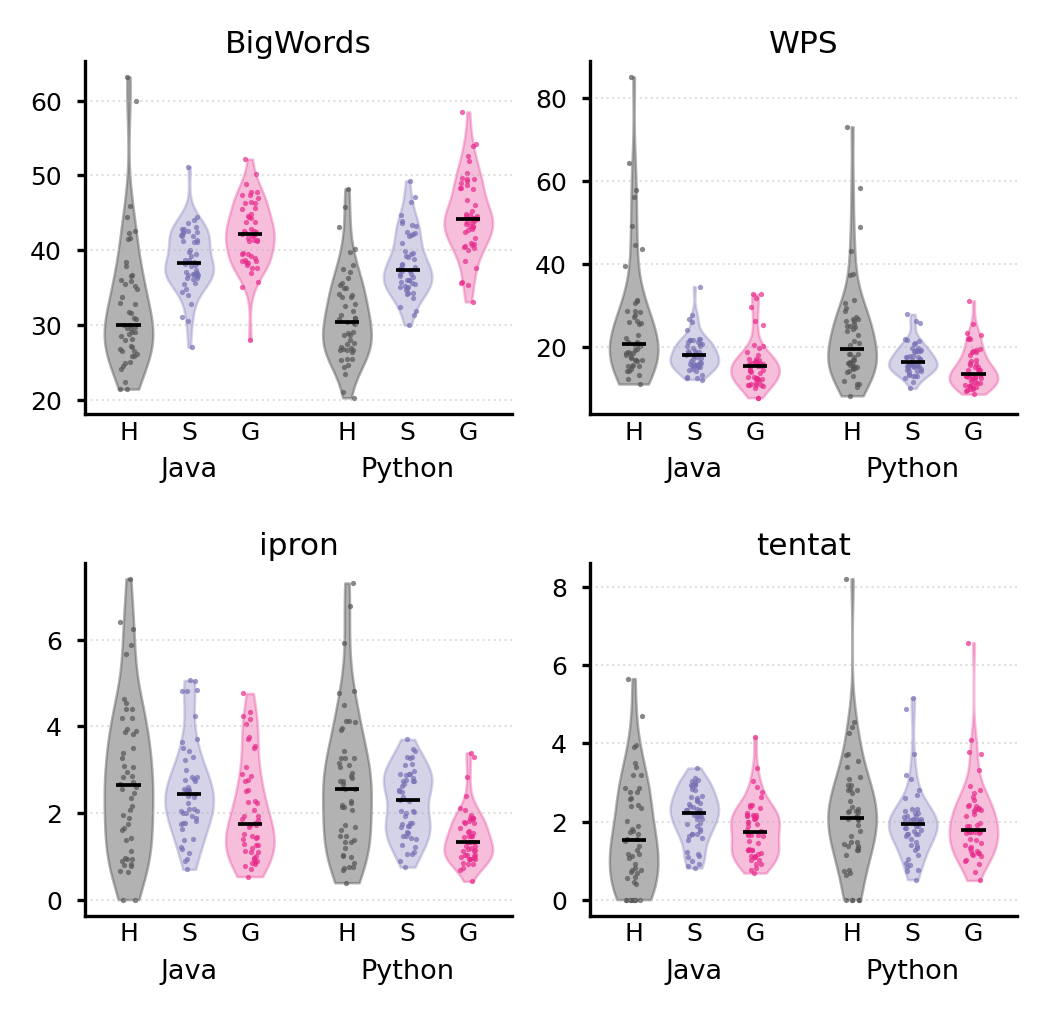
\includegraphics[width=0.85\columnwidth]{rq3_03_violin_compact.png}}
\caption{RQ3 distributions on the four dimensions behind the main results:
human (H), Claude Sonnet~5 (S) and GPT-5.6-terra (G), per ecosystem, $n=50$
each; bars are medians. \texttt{BigWords} shows the location shift (test~1);
\texttt{WPS}, \texttt{ipron} and \texttt{tentat} show the narrower spread of
generated documentation (test~4). The RQ4 authorship threshold
(\texttt{BigWords} $> 34.1$) lies between the human and generated medians.}
\label{fig:rq3violin}
\end{figure}

\begin{figure}[t]
\centerline{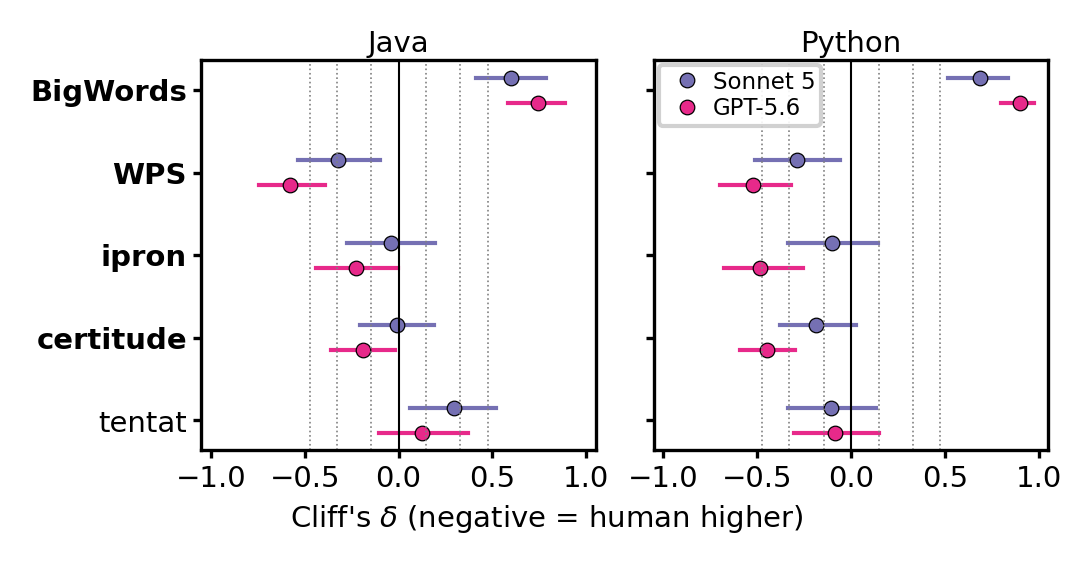
\includegraphics[width=\columnwidth]{rq3_test1_forest_compact.png}}
\caption{RQ3 test 1 on the construct-clean dimensions of Table~\ref{tbl:rq3t1}:
Cliff's $\delta$ with bootstrap 95\% CIs. Bold labels clear the decision rule
in at least one family; dotted lines mark the negligible/small/medium/large
boundaries. All 15 dimensions: Fig.~\ref{fig:rq3t1full}, Appendix~\ref{annex:figures}.}
\label{fig:rq3t1}
\end{figure}

\textbf{RQ3 is answered.} No axis-level claim was supported. On the Style axis, \texttt{BigWords} and \texttt{WPS} differed in opposite directions. For GPT on Java, \texttt{achieve} and \texttt{curiosity} both met the statistical rule, but their audited readings as creation verbs and how-to phrasing did not support a shared Drives interpretation. The following findings are therefore reported at dimension level. Under the evaluated production conditions, generated documentation had a higher proportion of long words than human documentation for the same libraries, consistently across both models and ecosystems. Human documentation also had higher \texttt{WPS} scores, although this difference met the decision rule only for GPT. Most model--ecosystem--dimension comparisons did not meet the decision rule, and no ecosystem difference in the human--model gap met it. The human--LLM gap on \texttt{BigWords} ($\delta = 0.60$--$0.90$) was larger than the Java--Python gap on that dimension ($\delta \approx 0.15$, $\eta^2 = 0.019$).

\section{RQ4: Ecosystem and Authorship Classification}
\label{sec:rq4}

\subsection{Method}

RQ1 tests each dimension in isolation. However, a classifer may expose joint structure across many dimensions where no univariate test can reveal, so RQ4 asks the question: given an unseen document's 15-dimensional profile, can its ecosystem be recovered?

Three classifiers (logistic regression, linear SVM, random forest) were trained on the duplication-corrected frame ($n=400$, 200 per ecosystem) using stratified 5-fold cross-validation repeated ten times. Features were standardised inside each training fold, so no test-fold information leaks into training. Chance is estimated by a permutation null: labels shuffled, model refit~\cite{ojala2010}. A classifier that beats the permutation baseline but falls short of the $0.75$ criterion (Section~\ref{sec:background}) indicates a signal that is detectable but not reliable.

\subsection{Ecosystem}

\textbf{The 0.75 criterion is not met.} The best model, the random forest, reaches macro-F1 $0.672$ against the target of $0.75$ (Table~\ref{tbl:rq4}, Appendix~\ref{annex:figures}).  All three models beat their permutation null ($p = 0.0099$). None of the three evaluated classifiers, including the nonlinear random forest, reached the specified reliability threshold.

These results complement RQ1: no dimension met the full decision rule in the corrected cross-ecosystem analysis, while the combined profile retained an ecosystem signal below the specified classification threshold.
\subsection{Authorship}

Ecosystem is one kind of origin; authorship is another, and the RQ3 corpus allows it to be tested. Human and generated documentation can be separated by a single threshold on a single dimension.

Fitted on all documents, the rule is \texttt{BigWords > 34.1} i.e, a document in which more than roughly a third of words run to seven characters or more, is classified as generated. Thresholds are learned inside each cross-validation fold on training rows only.
\begin{table}[htbp]
\caption{RQ4 authorship detection, $n=300$ (100 human, 200 generated).
Stratified 5-fold CV $\times$ 10 repeats, threshold relearned per fold.}
\label{tbl:rq4auth}
\begin{center}
\begin{tabular}{lcc}
\toprule
\textbf{Rule} & \textbf{macro-F1} & \textbf{Null} \\
\midrule
\texttt{BigWords} threshold   & \textbf{0.810} & 0.501 \\
\texttt{WPS} threshold        & 0.390 & 0.444 \\
Dispersion-centrality rule    & 0.373 & --- \\
\bottomrule
\end{tabular}
\end{center}
\end{table}

Table~\ref{tbl:rq4auth} reports the cross-validated scores; the feature's distributions appear in the \texttt{BigWords} panel of Fig.~\ref{fig:rq3violin} and, with the threshold, in Fig.~\ref{fig:rq4bw} (Appendix~\ref{annex:figures}). Accuracy is $0.839$, sensitivity $0.940$, specificity $0.670$ (permutation $p = 0.0099$), Matthews correlation $0.653$; threshold-free, average precision is $0.869$ against a no-skill $0.667$ and ROC AUC $0.853$. This rule is strong, but does have some certain limitations. It catches 94\% of generated documents, and its \emph{human} detections are correct 85\% of the time. However, it misflags around a third of genuine human documents, concentrated in short documents (42\% at 200--400 words against 24\% above 800), as a short README is dominated by identifiers and configuration keys, which usually are long tokens.

Additionally, there are two futher points which make this more than just a classification score. Firstly, the feature is \emph{not} a LIWC output: as shown in Section~\ref{sec:rq3}, it is recomputable from raw text, so the rule can be applied and audited without any licensed software. Secondly, the hypothesis that motivates this analysis is rejected. RQ3 shows that human documentation is more dispersed, meaning that for a document within one standard deviation of the human mean on both \texttt{BigWords} and \texttt{WPS}, it may be classified as machine-written. That rule scores $0.373$, below chance because the generated documents cluster \emph{inside} the human range rather than beside it, so most human documents are misclassified too. The dimensions on which humans spread more (\texttt{tentat}, \texttt{ipron}, \texttt{WPS}) are not the one on which the groups sit apart (\texttt{BigWords}). So, dispersion may describes the population as a whole but only a shifted centre can be used to classify an individual document.

\textbf{External validation.} An additional two checks were done on data that was not used to fit the rule. At the
fixed threshold, generations produced under five prompt conditions (baseline, anonymised name, length cap, paraphrase, explicit disclaimer) are flagged in 24 of 30 cases, 80\% recall. Imposing a length cap on the generated documents leads \texttt{BigWords} to the highest value of any of these variants, $40.4$. When told to be brief, the models compress into denser phrases rather than using plainer prose, meaning the long-word effect is not an artefact of unconstrained length. Additionally, after applying this rule to 2{,}400 human documents from the previous RQ1/RQ2 frames, this gives a 17.0\% false-positive rate (specificity 83.0\%), which is better than the 67\% measured within the RQ3 corpus. However, these documents are far longer with a median 4{,}415 words, and the human authorship is an assumption.

\textbf{RQ4 is thus answered.} The psycholinguistic profiles contained a detectable ecosystem signal, but none of the evaluated classifiers met the specified reliability threshold. The additional authorship analysis found that a single \texttt{BigWords} threshold distinguished human and generated documents in the evaluated corpus, although it misclassified approximately one-third of the human documents. This result concerns the documentation-production conditions studied here, rather than authorship independently of those conditions.

\section{Measurement Validity}
\label{sec:results-method-findings}

Three findings concern the interpretation of LIWC scores, the comparability of preprocessing, and the correspondence between paired documents. The audits and corrections changed which observed differences could support conclusions about documentation style.

\textbf{Selected affect scores could not be interpreted directly as emotional content.} In RQ1, the curated anger lexicon reproduced only a small portion of the LIWC \texttt{emo\_anger} score, leaving most of the audit's results unexplained. In RQ3, before preprocessing was corrected, generated documentation had higher negative-emotion and sadness scores, particularly for Java. The \texttt{emo\_neg} and \texttt{emo\_sad} scores correlated at $0.97$--$0.995$, while \texttt{emo\_pos} was near zero. Occurrences of the literal token ``java'' correlated with the sadness count ($r = 0.854$); documents without this token averaged $0.32\%$ on \texttt{emo\_sad}, compared with $4.59\%$ for documents containing twenty or more occurrences. Thus raising concerns about the interpretation of the affected dimensions as emotion content in this corpus.

\textbf{Asymmetric preprocessing altered the measured human--LLM differences.} Human READMEs had code removed during extraction, whereas generated output was initially scored without the same preprocessing. Source code accounted for roughly 36--56\% of generated text, compared with 0.8--2.4\% of human text, and 90\% of the generated ``java'' tokens occurred inside code blocks. Applying the same extraction function to generated text reduced residual code to 0.049\% corpus-wide. The Java \texttt{emo\_sad} score fell from $4.148\%$ to $0.024\%$, and the direction of the \texttt{WPS} difference reversed, due to code lines being parsed as long sentences. However, the \texttt{BigWords} findings remained unchanged. 

\textbf{Pairing required matching the software scope of both documents.}
\label{sec:readme-scope}
An audit identified 47 human READMEs that described a parent project rather than the sampled library (39/50 Java, 8/50 Python). This occured as the extractor fell back to the repository-root README when a module-level README was absent, introducing an ecosystem imbalance in document scope. Tables and unpunctuated lists also produced extreme \texttt{WPS} values. 

The corrected corpus required either a module-level README or a single-package repository, with at least 50 words post extraction. After these new requirements, replacement libraries were drawn in the original seeded order (Appendix~\ref{annex:proj-mgmt}). After rebuilding the corpus to $n=50$ per ecosystem, the \texttt{BigWords} finding remained unchanged, the \texttt{WPS} difference weakened, and all nine significant construct-valid dispersion comparisons showed greater spread in human documentation. No ecosystem difference in the human--model gap met the decision rule.
\section{Discussion}
\label{sec:results-discussion}

The main findings distinguish ecosystem differences from differences between human and generated documentation. Additionally, variation among libraries within an ecosystem accounts for most of the measured variance, and no cross-ecosystem dimension meets the full decision rule in the correct analysis. Regardless, classification detects an ecosystem signal below the specified reliability threshold. Additionally, Human and generated documentation differed consistently in terms of word length, with human documentation more dispersed in all nine significant construct-valid dispersion comparisons. These findings do not support a broad ecosystem level distinction under this study's criteria, nor do they establish that this remaining variation is due to indivudal authors.

But this does not contradict existing literature. Cagnoni et al.~\cite{cagnoni2020} find differing emotion distributions across Stack Overflow posts tagged with 26 programming languages, but those are \emph{conversational} artefacts, and Imran et al.~\cite{mohammad2022} report that emotion classifiers performed worse on a new GitHub dataset. But documentation may be a more constrained register, meaning genre constraints could suppress community-level variation which is visible in conversational text. This study which measures one genre, cannot settle this.

The human--LLM difference in \texttt{BigWords} was larger than the observed ecosystem difference on that dimension, while all nine significant construct-valid dispersion comparisons showed less variation in generated documentation. If these patterns extend to routine documentation generation, increased LLM use could reduce variation in some linguistic features. This possibility is consistent with Sourati et al.~\cite{sourati2026}, who report reduced writing-complexity variance in LLM-generated text outside software engineering. The present results concern dispersion in selected LIWC dimensions under a constrained generation setup; they do not establish a shift towards a single, more formal register.

\textbf{Reflection and lessons learned.} The most consequential errors in this project occurred during data handling, rather than in the statistics. Each of the three defects in Section~\ref{sec:results-method-findings} produced significant, replicated results prior to being discovered, and each was found during an manual inspection of an implausible value. In hindsight, the construct-validity audit and a single preprocessing function which both human and generated text shared should have been implemented before the first confirmatory run, and paired documents should have been checked for matching score before being generated. However, fixing the dimensions and decision rules in advance was useful, when effects shrank between the pilot and the confirmatory sample, this result could be reported without reinterpretation. The main lesson here is to treat any large or unexpected effect as a reason to look through the underlying documents before interpretation.

\subsection{Threats to Validity}

\emph{Construct validity.} Beyond the dimension-level failures reported in Section~\ref{sec:results-method-findings}, two structural risks still remain. Ten of the fifteen locked dimensions were rated mixed or register-shifted, which suggests the pilot's selection-by-discrimination may have favoured dimensions whose dictionaries overlap technical vocabulary: the criterion used to choose dimensions and the source of the artefacts are correlated. The axis rule also assumes that the dimensions are independent, which is incorrect. Nested dimensions break the rule such as (\texttt{emo\_sad} $\subset$ \texttt{emo\_neg} $\subset$ \texttt{emotion}). Thus, a single effect can satisfy the ``two dimensions, same direction'' requirement alone.

\emph{Internal validity.} RQ3's main limitation is information asymmetry. Human and LLMs differ not only as authors but in what they know: full project knowledge and adoption goals, against public API signatures alone. Therefore, the design then is measuring a documentation-production \emph{condition}, not a context-free effect of just authorship. For example, the model cannot write installation or licence sections. Creating fair conditions with the same fixed evidence for both human and LLM would give a more confirming result, something left for future work.

\emph{Domain labelling.} The domain tags in RQ2 come from a single rater, meaning there is no agreement statistic. 

\emph{External validity.} The study covers two ecosystems, two models, one genre and one prompt template, with $n=50$ per ecosystem for RQ3. Twelve human READMEs fall under 100 words after removing code, where percentage-based dimensions are unstable, and the Java sample under-represents large multi-module projects
(Section~\ref{sec:readme-scope}). Generated documents do not reproduce the real READMEs (maximum 8-gram containment $0.76\%$), although 19 of 200 contained fully qualified class names absent from the supplied API surface.

\section{Conclusion and Future Work}
\label{sec:conclusion}

This study examined documentation style across Java and Python libraries and between human and LLM-generated READMEs. No cross-ecosystem dimension met the full decision rule in the duplication-corrected corpus or the larger sample of $n=1000$ libraries per ecosystem. Most measured variation lay among libraries within ecosystems, although multivariate classification detected an ecosystem signal. In the paired README corpus, generated documentation contained a higher proportion of long words across both models and ecosystems. Sentence length was lower for generated documentation in both models, but met the decision rule only for GPT. No ecosystem difference in the human--model gap met the decision rule, and all nine significant construct-valid dispersion comparisons showed greater spread in human documentation.

Ecosystem classification reached a macro-F1 score of 0.672, which is below the set threshold of 0.85. However, in the authorship task, a \texttt{BigWords} threshold achieved a macro-F1 of 0.810, with 94\% sensitivity and 67\% specificity. From our prompt-variation task (when finding the initial prompt), after running the threshold on these, yielded a result of 24 of 30 generations being flagged with 80\% recall. Additionally, running on 2{,}400 additional documents (assumed to be human, the corpus for RQ1/2), 83\% specificity was achieved. These results support word length being a potential signal for human and generated documentation, under the conditions examined here, subject to false positives and the information asymmetry between the human authors and the models.

The methodological findings identify three threats to interpretation. Some LIWC dimensions could not be interpreted as their named psychological constructs in the evaluated technical text. Unequal code removal altered the measured human--LLM differences, including the direction of the sentence-length result. Finally, pairing a module's generated documentation with a repository-level README introduced a mismatch in scope, requiring further checks.

Future work from this study can follow two potential lines. Firstly, the task asymmetry in RQ3 could be addressed by giving the LLM the non-API content a human author would have had, which may isolate stylistic form from just an informational difference. Secondly, distinguisting the two mechanisms behind word length effect, do LLMs truly just normalise more, or do they echo the long identifiers supplied in the prompt.


\bibliographystyle{IEEEtran}
\bibliography{references}

\appendix
\section{Project Management Evidence}
\label{annex:proj-mgmt}

Hours were logged in an hour sheet throughout the project. A total of 304.0 hours was recorded against 300 planned. Table~\ref{tbl:tasks} lists the tasks as defined in the plan report with planned and actual hours, and Fig.~\ref{fig:hours} shows cumulative hours per week.

\subsection{Deviations from the Plan}

The following deviations are substantive and each has a documented rationale.

\begin{enumerate}
\item \textbf{Documentation source changed.} The plan specified crawling hosted documentation sites, but instead moved to cloning repositories and using the documentation supplied in the repository (README and docs/trees). First for java, and then for both ecosystems, such that every library was acquired using the same procedure. Thus, the research questions are rewording from API documentation to library documentation.
\item \textbf{Success criteria replaced.} The plan's criteria (a significant
Kruskal--Wallis result for RQ1/RQ2, a significant Wilcoxon result for RQ3, and
accuracy above a random baseline for RQ4) were replaced before the confirmatory
collection by the decision rule of Section~\ref{sec:rule} and the macro-F1
$0.75$ criterion, which combine significance with a minimum effect size.
\item \textbf{Third ecosystem dropped.} The planned third ecosystem
(JavaScript) was removed from the confirmatory scope. Additionally, a later attempt to obtain a different ecosystem (Haskell) was also dropped, as Haskell only drew 900 packages and meant the entire Hackage population only resulted in 85 usable libraries. (325 had no clonable repository and 490 fell below 500 words)
\item \textbf{Corpus scale increased, then RQ3 scale reduced.} RQ1 was
re-estimated at $n=1000$/ecosystem following supervisor feedback. RQ3 generation
was reduced from the full corpus to a seeded 50 per ecosystem on cost grounds.
\item \textbf{RQ3 corpus redrawn after the README scoping defect}
(Section~\ref{sec:readme-scope}). Two inclusion rules were added, defined on
the repository structure and applied without reference to any LIWC score. The draw was continued from the original seeded order (into the frame's reserve pool, and then into the resulting 2000 frame used for RQ1/RQ2). There are two significant consequences from this. The Java sample now spans two sampling frames (both built via the same machinery under the same filters), and libraries which do not ship a module-level README are excluded, which may under represent large projects.
\item \textbf{Confirmatory stage added.} Not in the original plan. A pilot,
a locked dimension list, and a fixed decision rule were introduced after the
pilot showed 13 of 15 dimensions ``passing''. A result that would not have been
interpretable without the confirmatory stage.
\item \textbf{RQ2's exploratory sweep over the remaining 44 dimensions was
descoped}, as no dimension in the committed set had met the decision rule.
\item \textbf{RQ4 completed, with a broader scope than planned.} The
classification analysis was run in full (three models, permutation and
majority-class baselines, domain classification). The macro-F1
threshold of 0.75, however, was fixed under a three-ecosystem design that was
never executed.
\end{enumerate}

\subsection{Task Decomposition and Time Tracking}

Table~\ref{tbl:tasks} lists the tasks as defined in the plan report, with
planned (Est.) and logged (Act.) hours, followed by unplanned work. Tasks more
than 30\% above or below their estimate are explained below the table.

\begin{table}[htbp]
\caption{Plan-report tasks with estimated and actual hours. Dev.\ is the
deviation from the estimate; N/A marks work after the report due date.}
\label{tbl:tasks}
\centering
\footnotesize
\begin{tabular}{@{}l p{0.52\columnwidth} r r r@{}}
\toprule
\textbf{M} & \textbf{Task} & \textbf{Est.} & \textbf{Act.} & \textbf{Dev.} \\
\midrule
M0 & Background research and literature review          & 10   & 32.2 & +222\% \\
M0 & Plan report writing                                & 12.5 & 11.2 & $-$10\% \\
\midrule
M1 & Define ecosystems, genre, scale, sampling criteria & 10   & 11.2 & +12\% \\
M1 & Sample libraries via popularity ranking; validate doc URLs & 10 & 5.7 & $-$43\% \\
M1 & Build HTML crawler with encoding normalisation     & 15   & 16.7 & +11\% \\
M1 & Build pre-processor: strip markup, partition sections & 20 & 14.8 & $-$26\% \\
\midrule
M2 & LIWC batch processing and output validation        & 15   & 15.2 & +2\% \\
M2 & Structural feature extraction (sentence length, passive voice) & 15 & 0 & $-$100\% \\
M2 & RQ1 analysis scripts and visualisations            & 20   & 23.3 & +17\% \\
M2 & RQ2 analysis scripts and variance visualisations   & 15   & 4.0  & $-$73\% \\
\midrule
M3 & Build AI corpus: select APIs, generate docs via LLM & 20  & 21.5 & +8\% \\
M3 & RQ3 divergence analysis and interpretation         & 17   & 11.0 & $-$35\% \\
\midrule
M4 & Demo 1: slides and live pipeline demonstration     & 10   & 15.5 & +55\% \\
\midrule
M5 & RQ4 similarity tool: cosine scorer and evaluation  & 25   & 0    & $-$100\% \\
M5 & Optional: classifier training and cross-validation & 15   & 8.3  & $-$44\% \\
\midrule
M6 & Demo 2: results walkthrough and tool demonstration & 10   & N/A  & --- \\
M7 & Stretch: AI detector training and evaluation       & 25   & 3.8  & $-$85\% \\
M8 & Final report: draft, revise, proofread             & 25   & 27.9 & +12\% \\
M9 & Showcase preparation                               & 10   & N/A  & --- \\
\midrule
-- & \emph{Unplanned:} supervisor meetings, preparation and summaries & -- & 15.1 & -- \\
-- & \emph{Unplanned:} pilot dimension selection and construct-validity audit & -- & 25.5 & -- \\
-- & \emph{Unplanned:} defect diagnosis and corpus corrections & -- & 35.5 & -- \\
-- & \emph{Unplanned:} abandoned explorations (Haskell, tutorial genre) & -- & 5.5 & -- \\
\midrule
\multicolumn{2}{r}{\textbf{Total}} & \textbf{300} & \textbf{304.0} & +1\% \\
\bottomrule
\end{tabular}
\end{table}

\textbf{Deviations above 30\%.}
\emph{Background research} (+222\%) included LIWC and statistical reading and the
systematic literature search re-run on Scopus for this report.
\emph{Library sampling} ($-$43\%) used a seeded draw from the ecosyste.ms index
rather than a popularity ranking, and repository-based acquisition removed the
need to validate hosted documentation URLs.
\emph{Structural feature extraction} was dropped: sentence length is provided by
LIWC's \texttt{WPS}, and passive voice was not among the selected dimensions.
\emph{RQ2} ($-$73\%) and \emph{RQ3 analysis} ($-$35\%) reused the RQ1 data and the
shared statistics module; the time spent correcting RQ3 is recorded in the
defect row.
\emph{Demo 1} (+55\%) required more slide and script preparation than estimated.
The \emph{cosine similarity tool} was replaced by the classification approach,
which evaluates ecosystem prediction directly with standard metrics; that task
($-$44\%) reused shared cross-validation routines.
The \emph{AI detector} stretch goal was achieved ($-$85\%), the reason for the short time is a single-threshold
rule required not a lot of training time, and its corpus was built under the RQ3 tasks.
\emph{Unplanned work} totalled 81.6 hours, mainly focusing on corpus-defect diagnosis and
correction (35.5 h) and the pilot dimension selection and construct-validity
audit (25.5 h), which were absorbed by the tasks that finished under estimate.
The plan's 23 weeks are teaching weeks; mapped onto the calendar
(Fig.~\ref{fig:hours}), effective hours trailed the plan through Semester One
(130.5 h against 168 h by week 15), partly recovered through work during the
mid-year break, and finished at 304.0 h against 300 h.

\begin{figure}[htbp]
\centering
\begin{tikzpicture}
\begin{axis}[
  width=\columnwidth, height=5.2cm,
  xlabel={Calendar week (week 1 = 16 February)}, ylabel={Cumulative hours},
  xmin=1, xmax=34, ymin=0, ymax=320,
  xtick={1,5,10,15,20,25,30,34}, ytick={0,100,200,300},
  grid=major, grid style={dashed,gray!30},
  legend pos=north west, legend style={font=\footnotesize},
  tick label style={font=\footnotesize}, label style={font=\footnotesize},
]
\fill[gray!15] (axis cs:6.5,0)  rectangle (axis cs:9.5,320);
\fill[gray!15] (axis cs:15.5,0) rectangle (axis cs:21.5,320);
\fill[gray!15] (axis cs:27.5,0) rectangle (axis cs:29.5,320);
\addplot[blue, mark=*, mark size=1pt] coordinates {
(1,0)(2,10)(3,22)(4,34)(5,52)(6,70)(7,70)(8,70)(9,70)(10,88)(11,106)
(12,118)(13,136)(14,152)(15,168)(16,168)(17,168)(18,168)(19,168)(20,168)
(21,168)(22,184)(23,196)(24,208)(25,220)(26,232)(27,248)(28,248)(29,248)
(30,264)(31,274)(32,284)(33,292)(34,300)};
\addlegendentry{Expected (plan)}
\addplot[red, mark=square*, mark size=1pt] coordinates {
(1,0)(2,0)(3,9.9)(4,20.8)(5,30.3)(6,44.5)(7,48.5)(8,48.5)(9,48.5)(10,64.5)
(11,70.0)(12,84.0)(13,103.5)(14,120.5)(15,130.5)(16,134.0)(17,137.3)(18,138.3)
(19,140.8)(20,142.5)(21,151.5)(22,165.3)(23,180.2)(24,194.2)(25,204.7)
(26,220.2)(27,231.9)(28,231.9)(29,231.9)(30,236.8)(31,254.5)(32,271.8)
(33,281.7)(34,304.0)};
\addlegendentry{Effective (logged)}
\end{axis}
\end{tikzpicture}
\caption{Expected and effective cumulative hours. The plan's 23 teaching weeks
are mapped onto calendar weeks; shaded weeks are university breaks, during
which no hours were planned.}
\label{fig:hours}
\end{figure}


\section{Literature Search Detail}
\label{annex:search}

Supporting evidence for Section~\ref{sec:related}, which states the method, criteria
and funnel. Nothing here is required to follow the argument.

\subsection{Two Searches, Reported Separately}

The \textbf{primary search} (May 2026, ten sources) produced the included set:
approximately 1{,}400 records retrieved, roughly 950 after deduplication, 70
advanced to full text, 25 retained and six added by citation chaining, giving 31;
an audit then removed four, leaving 27. The \textbf{verification} (September
2026, Scopus only) re-ran the same sixteen strings to obtain exact, reproducible
counts, returning 1{,}830 records and 1{,}624 unique. only 9 of the 27 included works appear in the 1{,}624, the
other 18 being books, theses and reports Scopus does not index, or papers these
strings do not retrieve. A third, \textbf{supplementary} search, claim-driven
rather than systematic, contributed twelve further references cited for
specific claims.

\subsection{Per-String Retrieval}

\begin{table}[htbp]
\caption{Scopus, \texttt{TITLE-ABS-KEY}. Filters inside each
query: \texttt{LANGUAGE(english)} and document type article, conference paper,
review or chapter. No date filter at retrieval, so the publication-window
criterion is applied at screening rather than silently.}
\label{tbl:search}
\begin{center}
\begin{tabular}{llr}
\toprule
\textbf{String} & \textbf{Intersection} & \textbf{Records} \\
\midrule
1a & LIWC $\times$ ``software engineering''      & 7 \\
1b & LIWC $\times$ software                      & 414 \\
2a & API documentation $\times$ quality          & 95 \\
2b & API documentation $\times$ developers       & 264 \\
2c & Software documentation $\times$ style       & 112 \\
3a & LLM $\times$ LIWC / psycholinguistic        & 109 \\
3b & LLM $\times$ stylometric $\times$ detection & 546 \\
3c & LLM $\times$ documentation $\times$ comparison & 126 \\
4a & Developer $\times$ emotion $\times$ LIWC    & 4 \\
4b & Sentiment $\times$ SE $\times$ SO/GitHub    & 60 \\
4c & Developer communication $\times$ linguistic & 5 \\
5a & Register variation $\times$ corpus linguistics & 45 \\
5b & Biber $\times$ register $\times$ MD analysis & 37 \\
5c & Register variation $\times$ programming     & 1 \\
6a & Linguistic behaviour $\times$ OSS           & 2 \\
6b & Ecosystem $\times$ community $\times$ style & 3 \\
\midrule
\multicolumn{2}{l}{By round: R1 421, R2 471, R3 781, R4 69, R5 83, R6 5} & \\
\multicolumn{2}{l}{Total with overlap} & 1{,}830 \\
\multicolumn{2}{l}{\textbf{Unique after combining with OR}} & \textbf{1{,}624} \\
\multicolumn{2}{l}{Overlap} & 206 (11.3\%) \\
\bottomrule
\end{tabular}
\end{center}
\end{table}

\subsection{Sparse Topic Intersections}

The sparse intersections indicate how rarely the retrieved literature combines these topics: register variation intersected with programming or technical documentation returned \textbf{1} record; linguistic behaviour in open source with social status, \textbf{2}; ecosystem with community writing style, \textbf{3}; developer emotion with LIWC, \textbf{4}; developer communication with linguistic analysis, \textbf{5}; and LIWC with ``software engineering'', \textbf{7}. These show where the indexed literature is thin, not that no relevant prior work exists.

\subsection{ Screening of the Scopus Set}

The 1{,}624 records were put through a two-pass triage that applies certain rules
and records which fired for every record. Abstracts were present for 1{,}620 of 1{,}624, making this
title-\emph{and}-abstract screening.

\begin{table}[htbp]
\caption{Triage of the sources. Pass 1 removes records
failing a stated criterion irrespective of topic; pass 2 removes eligible but
off-topic records. The buckets are triage, not decisions.}
\label{tbl:triage}
\begin{center}
\begin{tabular}{lr}
\toprule
\textbf{Stage} & \textbf{Records} \\
\midrule
Retrieved & 1{,}624 \\
\quad less duplicate DOIs (E2) & $-$2 \\
\quad less published before 2010 (I2) & $-$84 \\
\quad less out-of-scope domain (E4) & $-$492 \\
\quad\quad \emph{clinical 281, social 142, education 34,} & \\
\quad\quad \emph{finance 19, other NLP 16} & \\
\midrule
Eligible after pass 1 & 1{,}046 \\
\quad less no software $+$ language signal & $-$442 \\
\midrule
\textbf{Advance to manual screening} & \textbf{604} \\
\bottomrule
\end{tabular}
\end{center}
\end{table}


\section{Supplementary Tables and Figures}
\label{annex:figures}

These tables and figures expand results already stated numerically in
the body; none carries a claim of its own.

\begin{table}[htbp]
\caption{RQ4 ecosystem classification, $n=400$ (200 Java / 200 Python).}
\label{tbl:rq4}
\begin{center}
\begin{tabular}{lccc}
\toprule
\textbf{Model} & \textbf{macro-F1} & \textbf{Held-out 20\%} & \textbf{Null} \\
\midrule
Logistic regression & 0.616 & 0.612 & 0.499 \\
Linear SVM          & 0.610 & 0.600 & 0.498 \\
Random forest       & \textbf{0.672} & 0.674 & 0.500 \\
\midrule
Majority-class floor & 0.333 & --- & --- \\
Target (fixed in advance) & 0.75 & --- & --- \\
\bottomrule
\end{tabular}
\end{center}
\end{table}

\begin{table}[htbp]
\caption{Variance decomposition, confirmatory corpus ($n=200$ per ecosystem,
duplication-corrected). $\eta^2$ is the share of total variance attributable to
ecosystem membership.}
\label{tbl:rq2var}
\begin{center}
\begin{tabular}{lrr}
\toprule
\textbf{Dimension} & \textbf{$\eta^2$ between} & \textbf{\% variance within} \\
\midrule
\texttt{ipron}     & 0.032 & 96.8 \\
\texttt{emo\_anger}& 0.030 & 97.0 \\
\texttt{conflict}  & 0.024 & 97.6 \\
\texttt{tentat}    & 0.020 & 98.0 \\
\texttt{BigWords}  & 0.019 & 98.1 \\
\multicolumn{3}{c}{\emph{\ldots remaining 9 dimensions all below 0.017\ldots}} \\
\texttt{Tone}      & 0.000 & 100.0 \\
\midrule
\textbf{mean}      & \textbf{0.012} & \textbf{98.8} \\
\bottomrule
\end{tabular}
\end{center}
\end{table}

\begin{figure}[htbp]
\centerline{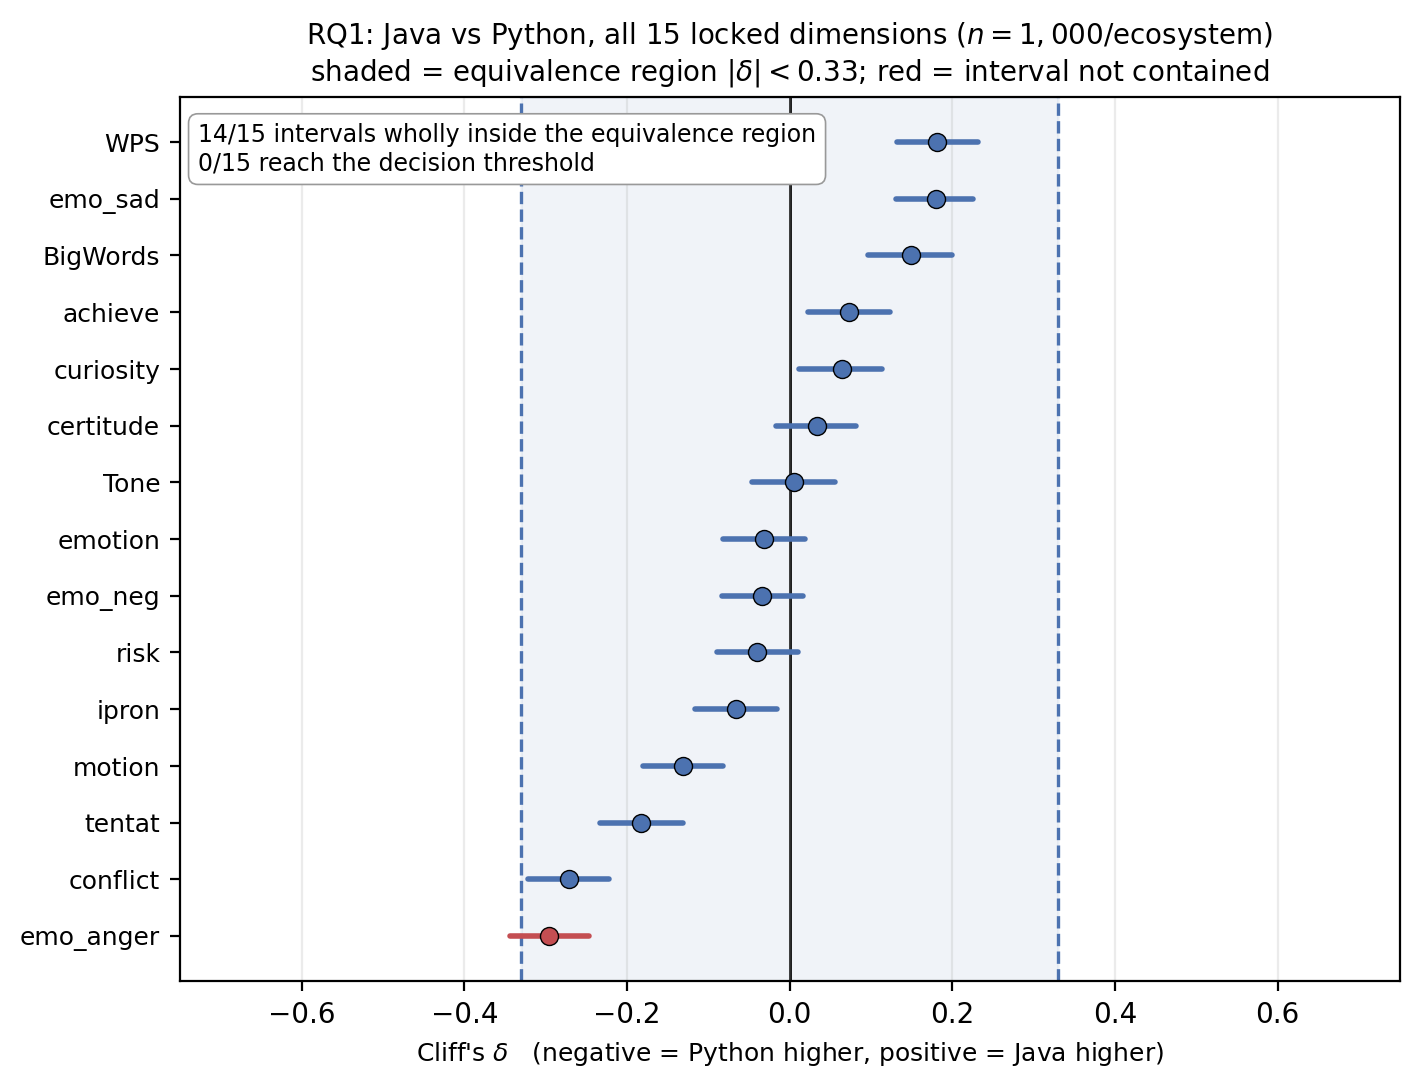
\includegraphics[width=\columnwidth]{rq1_forest.png}}
\caption{RQ1. Cliff's $\delta$ for Java versus Python across the 15 locked
dimensions, with bootstrap 95\% CIs. Dashed lines mark the
$|\delta| = 0.33$ threshold. No point estimate reaches this threshold;
the confidence interval for \texttt{emo\_anger} extends beyond it.}
\label{fig:rq1}
\end{figure}

\begin{figure}[htbp]
\centerline{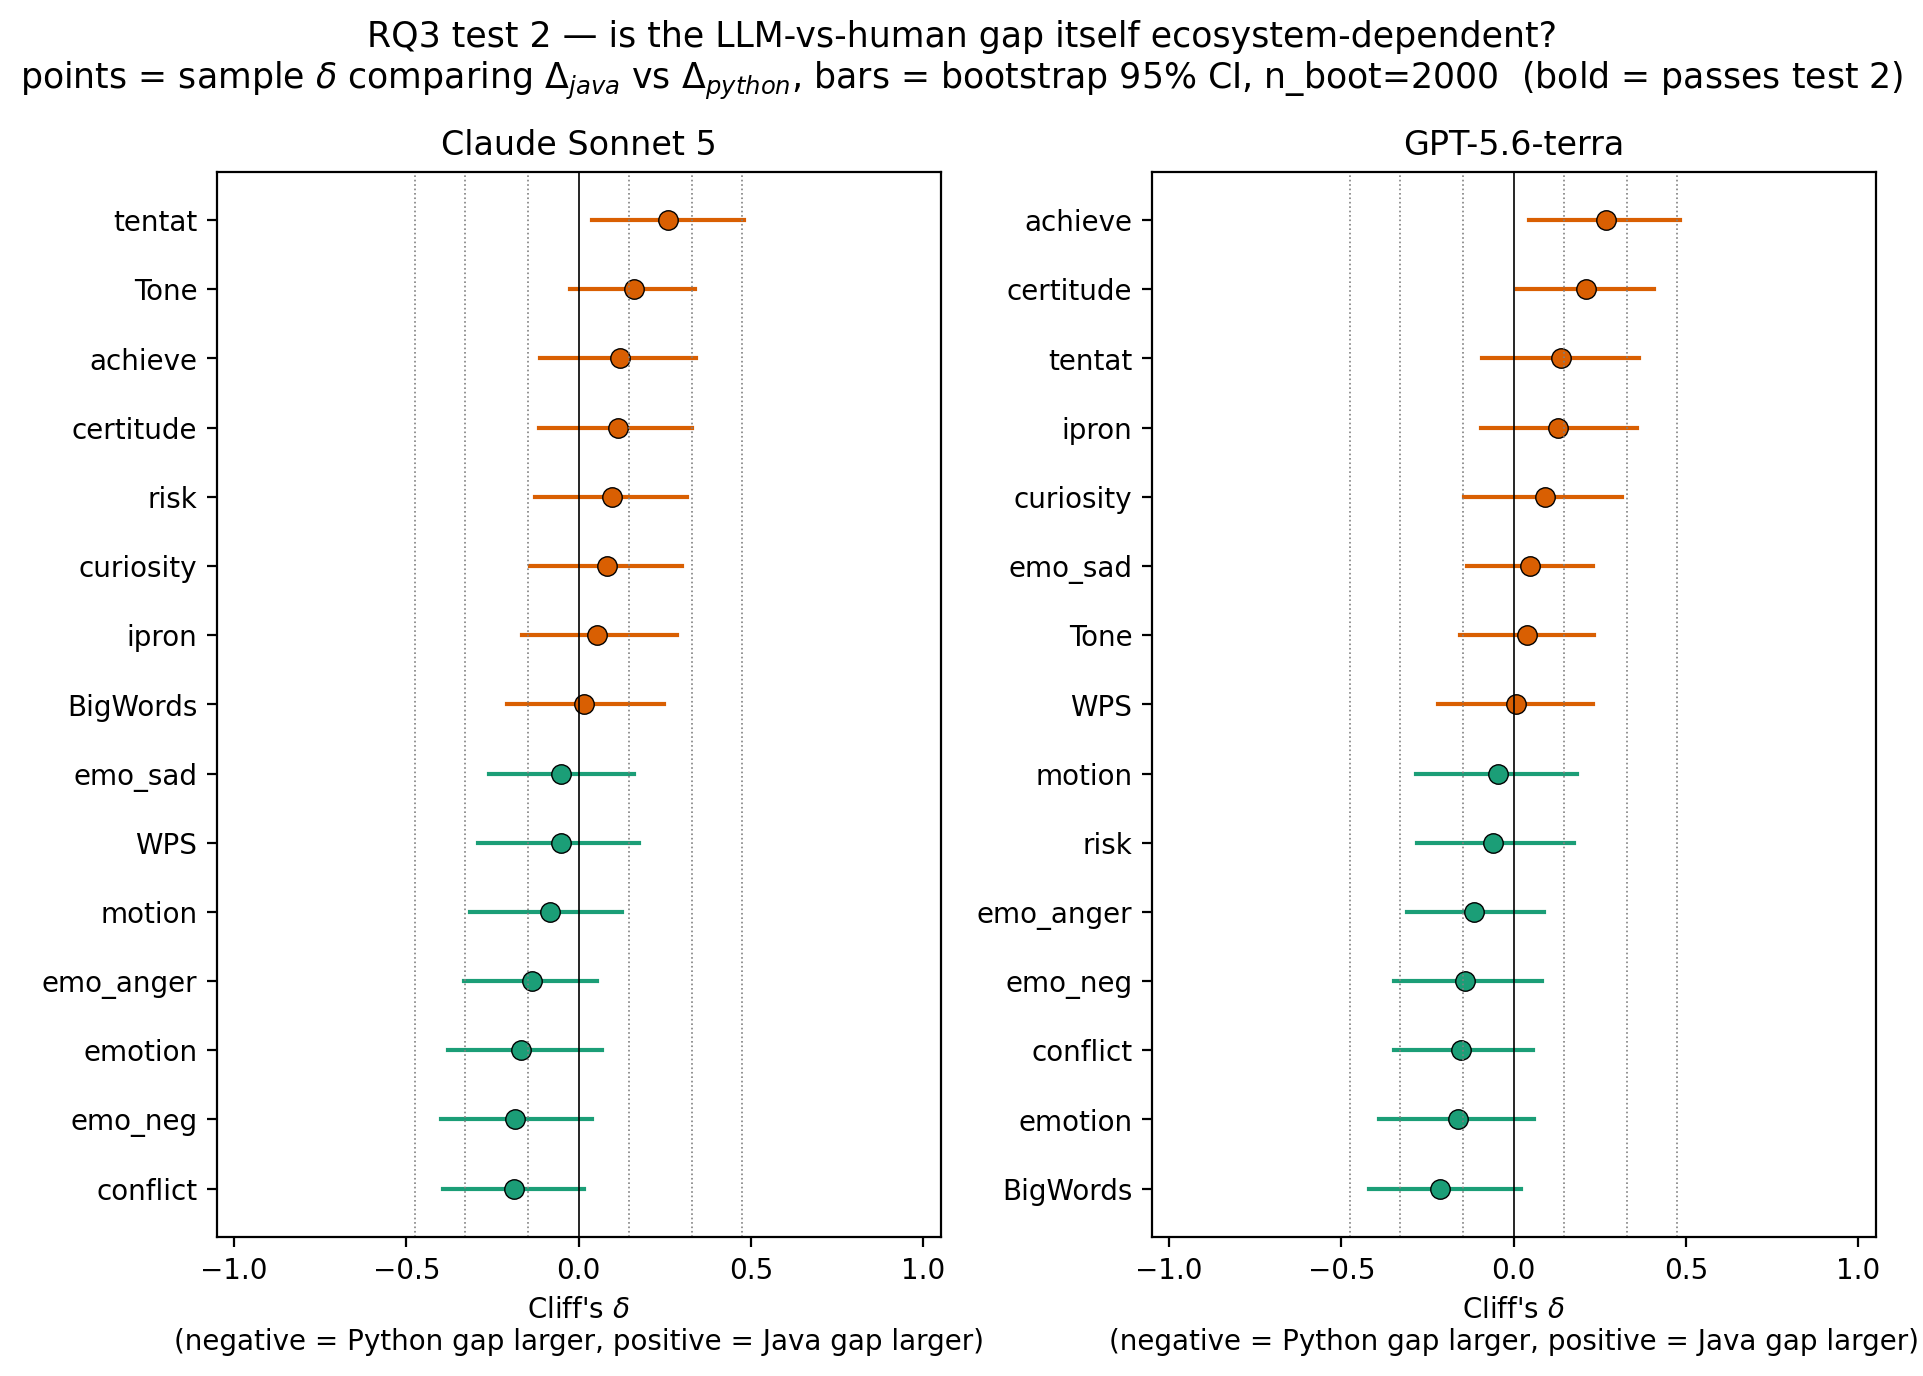
\includegraphics[width=\columnwidth]{rq3_test2_forest.png}}
\caption{RQ3 test 2. Cliff's $\delta$ for the Java-versus-Python comparison of
the human--model gap, bootstrap 95\% CIs. Every interval spans zero.}
\label{fig:supp}
\end{figure}

\begin{figure}[htbp]
\centerline{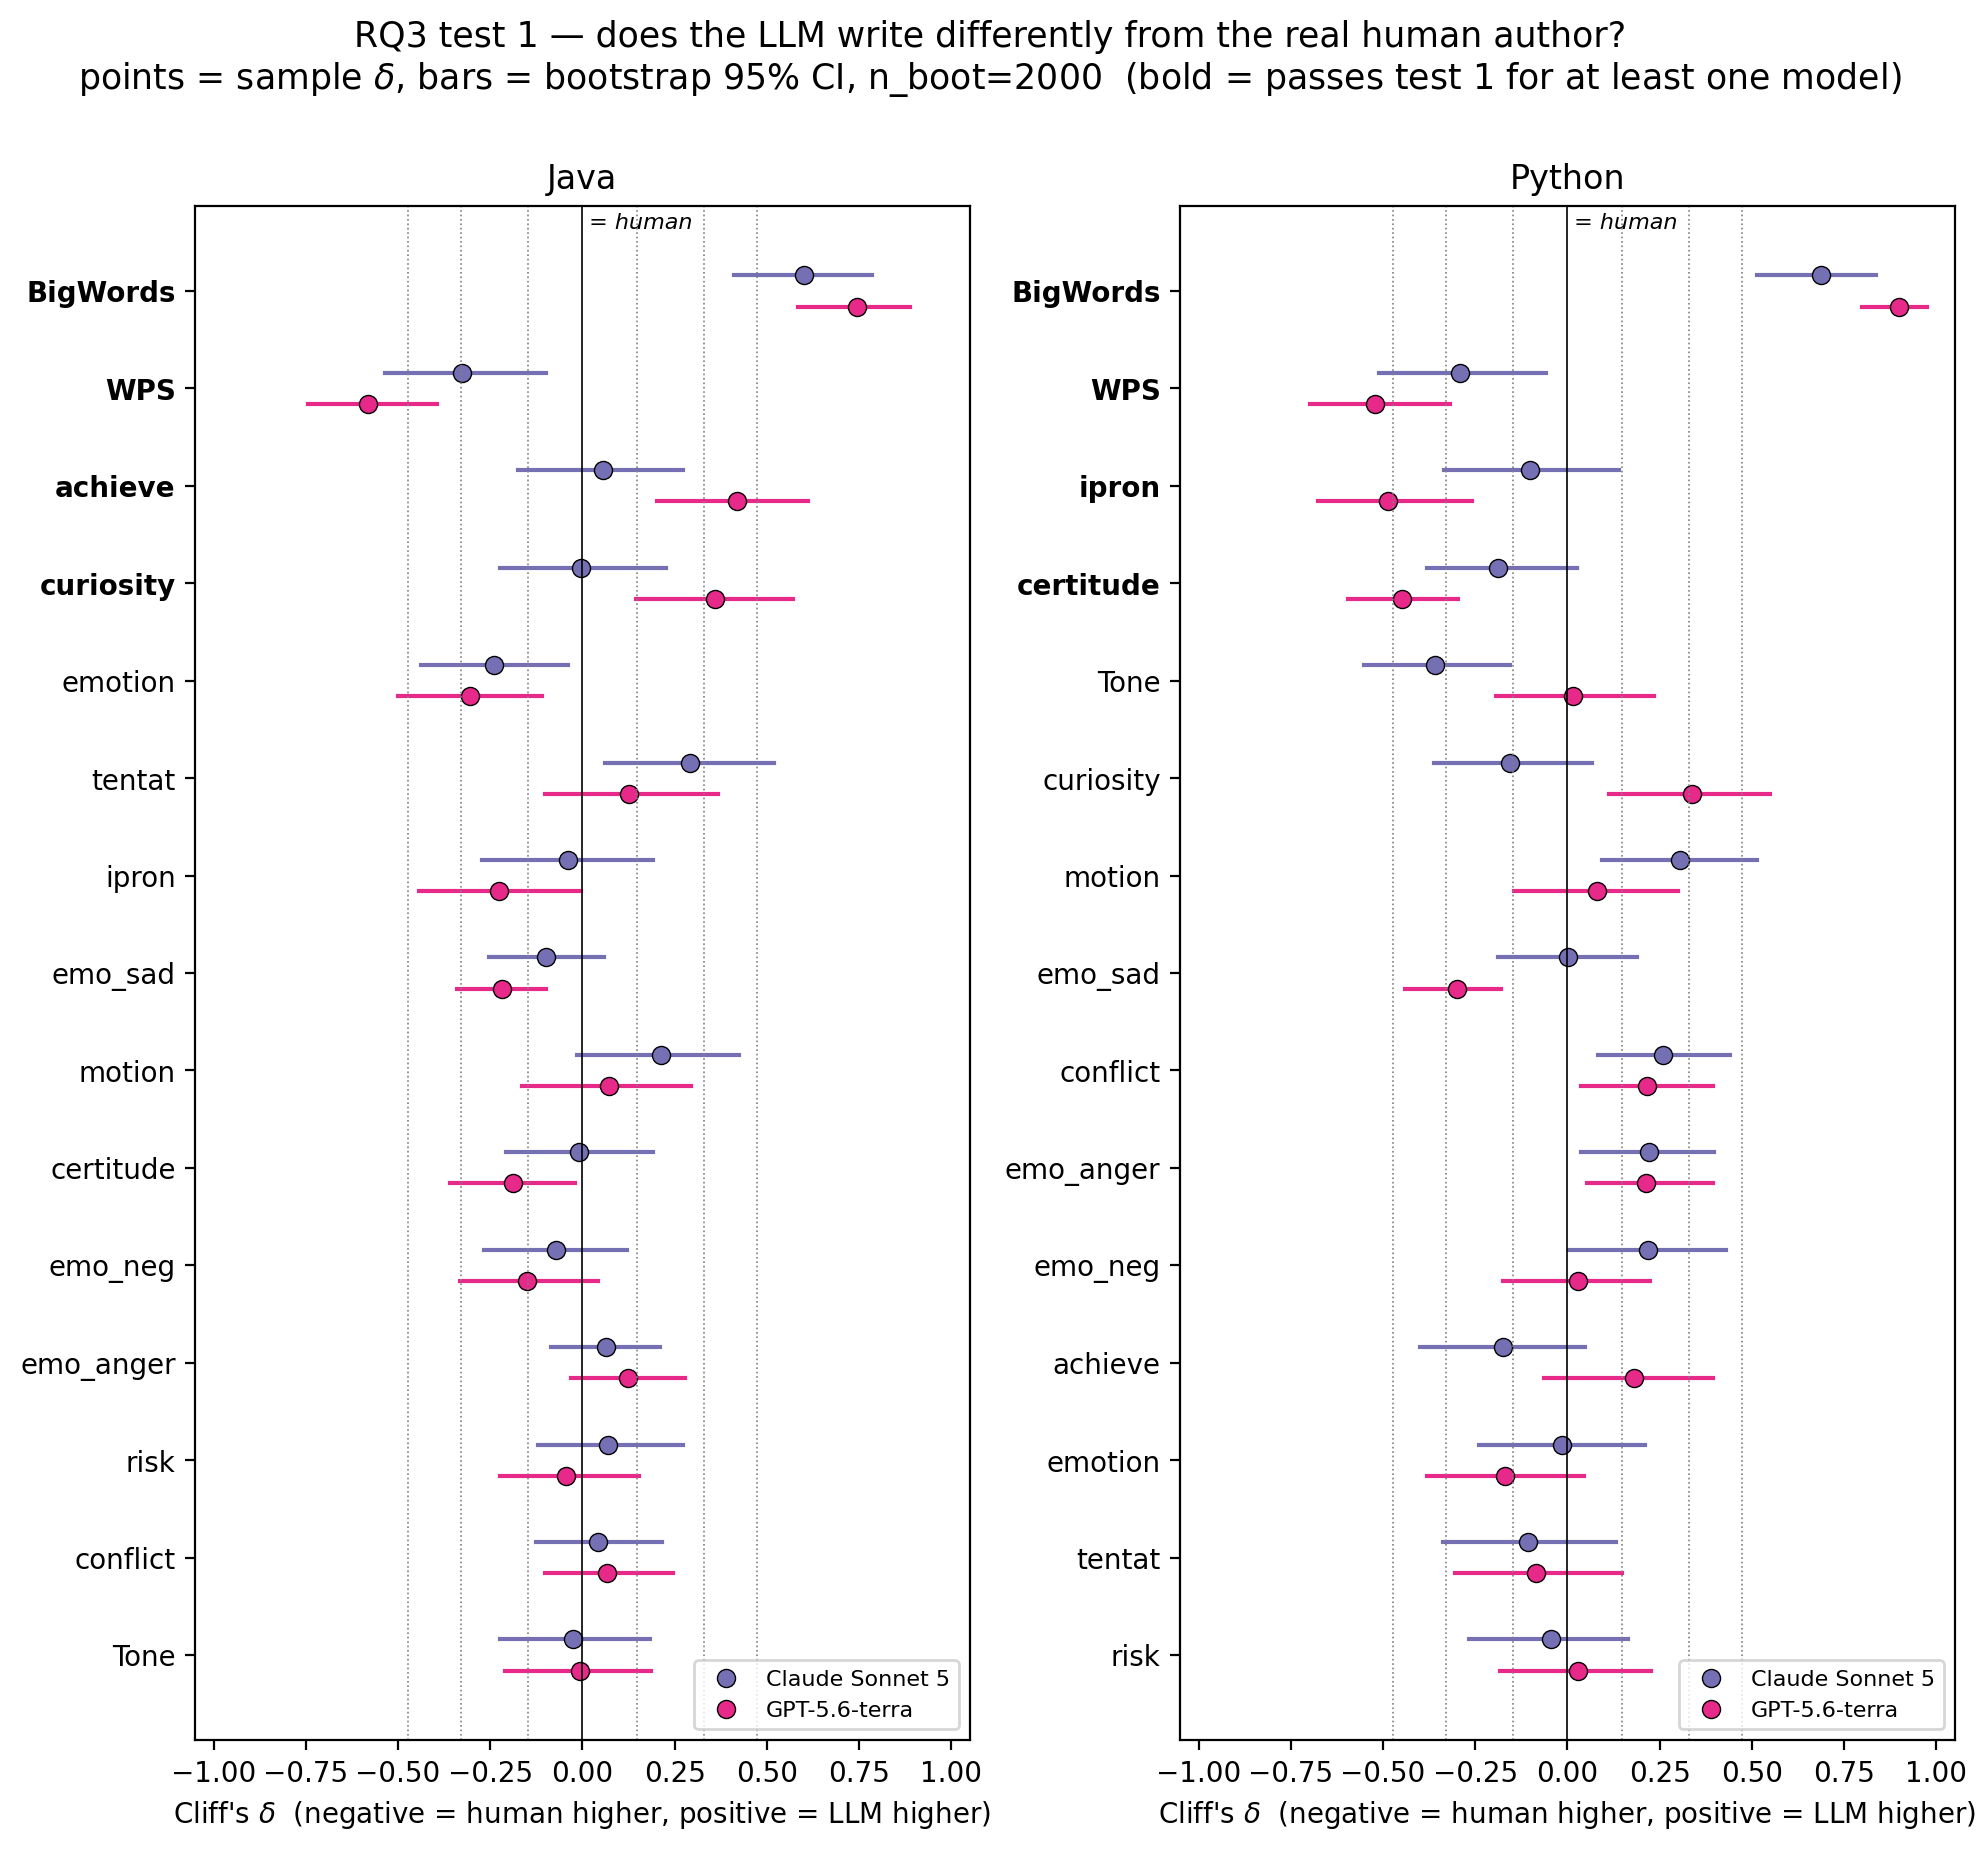
\includegraphics[width=\columnwidth]{rq3_test1_forest.png}}
\caption{RQ3 test 1, all 15 locked dimensions: Cliff's $\delta$ with bootstrap
95\% CIs, by ecosystem and model. Bold labels clear the decision rule.}
\label{fig:rq3t1full}
\end{figure}

\begin{figure*}[htbp]
\centerline{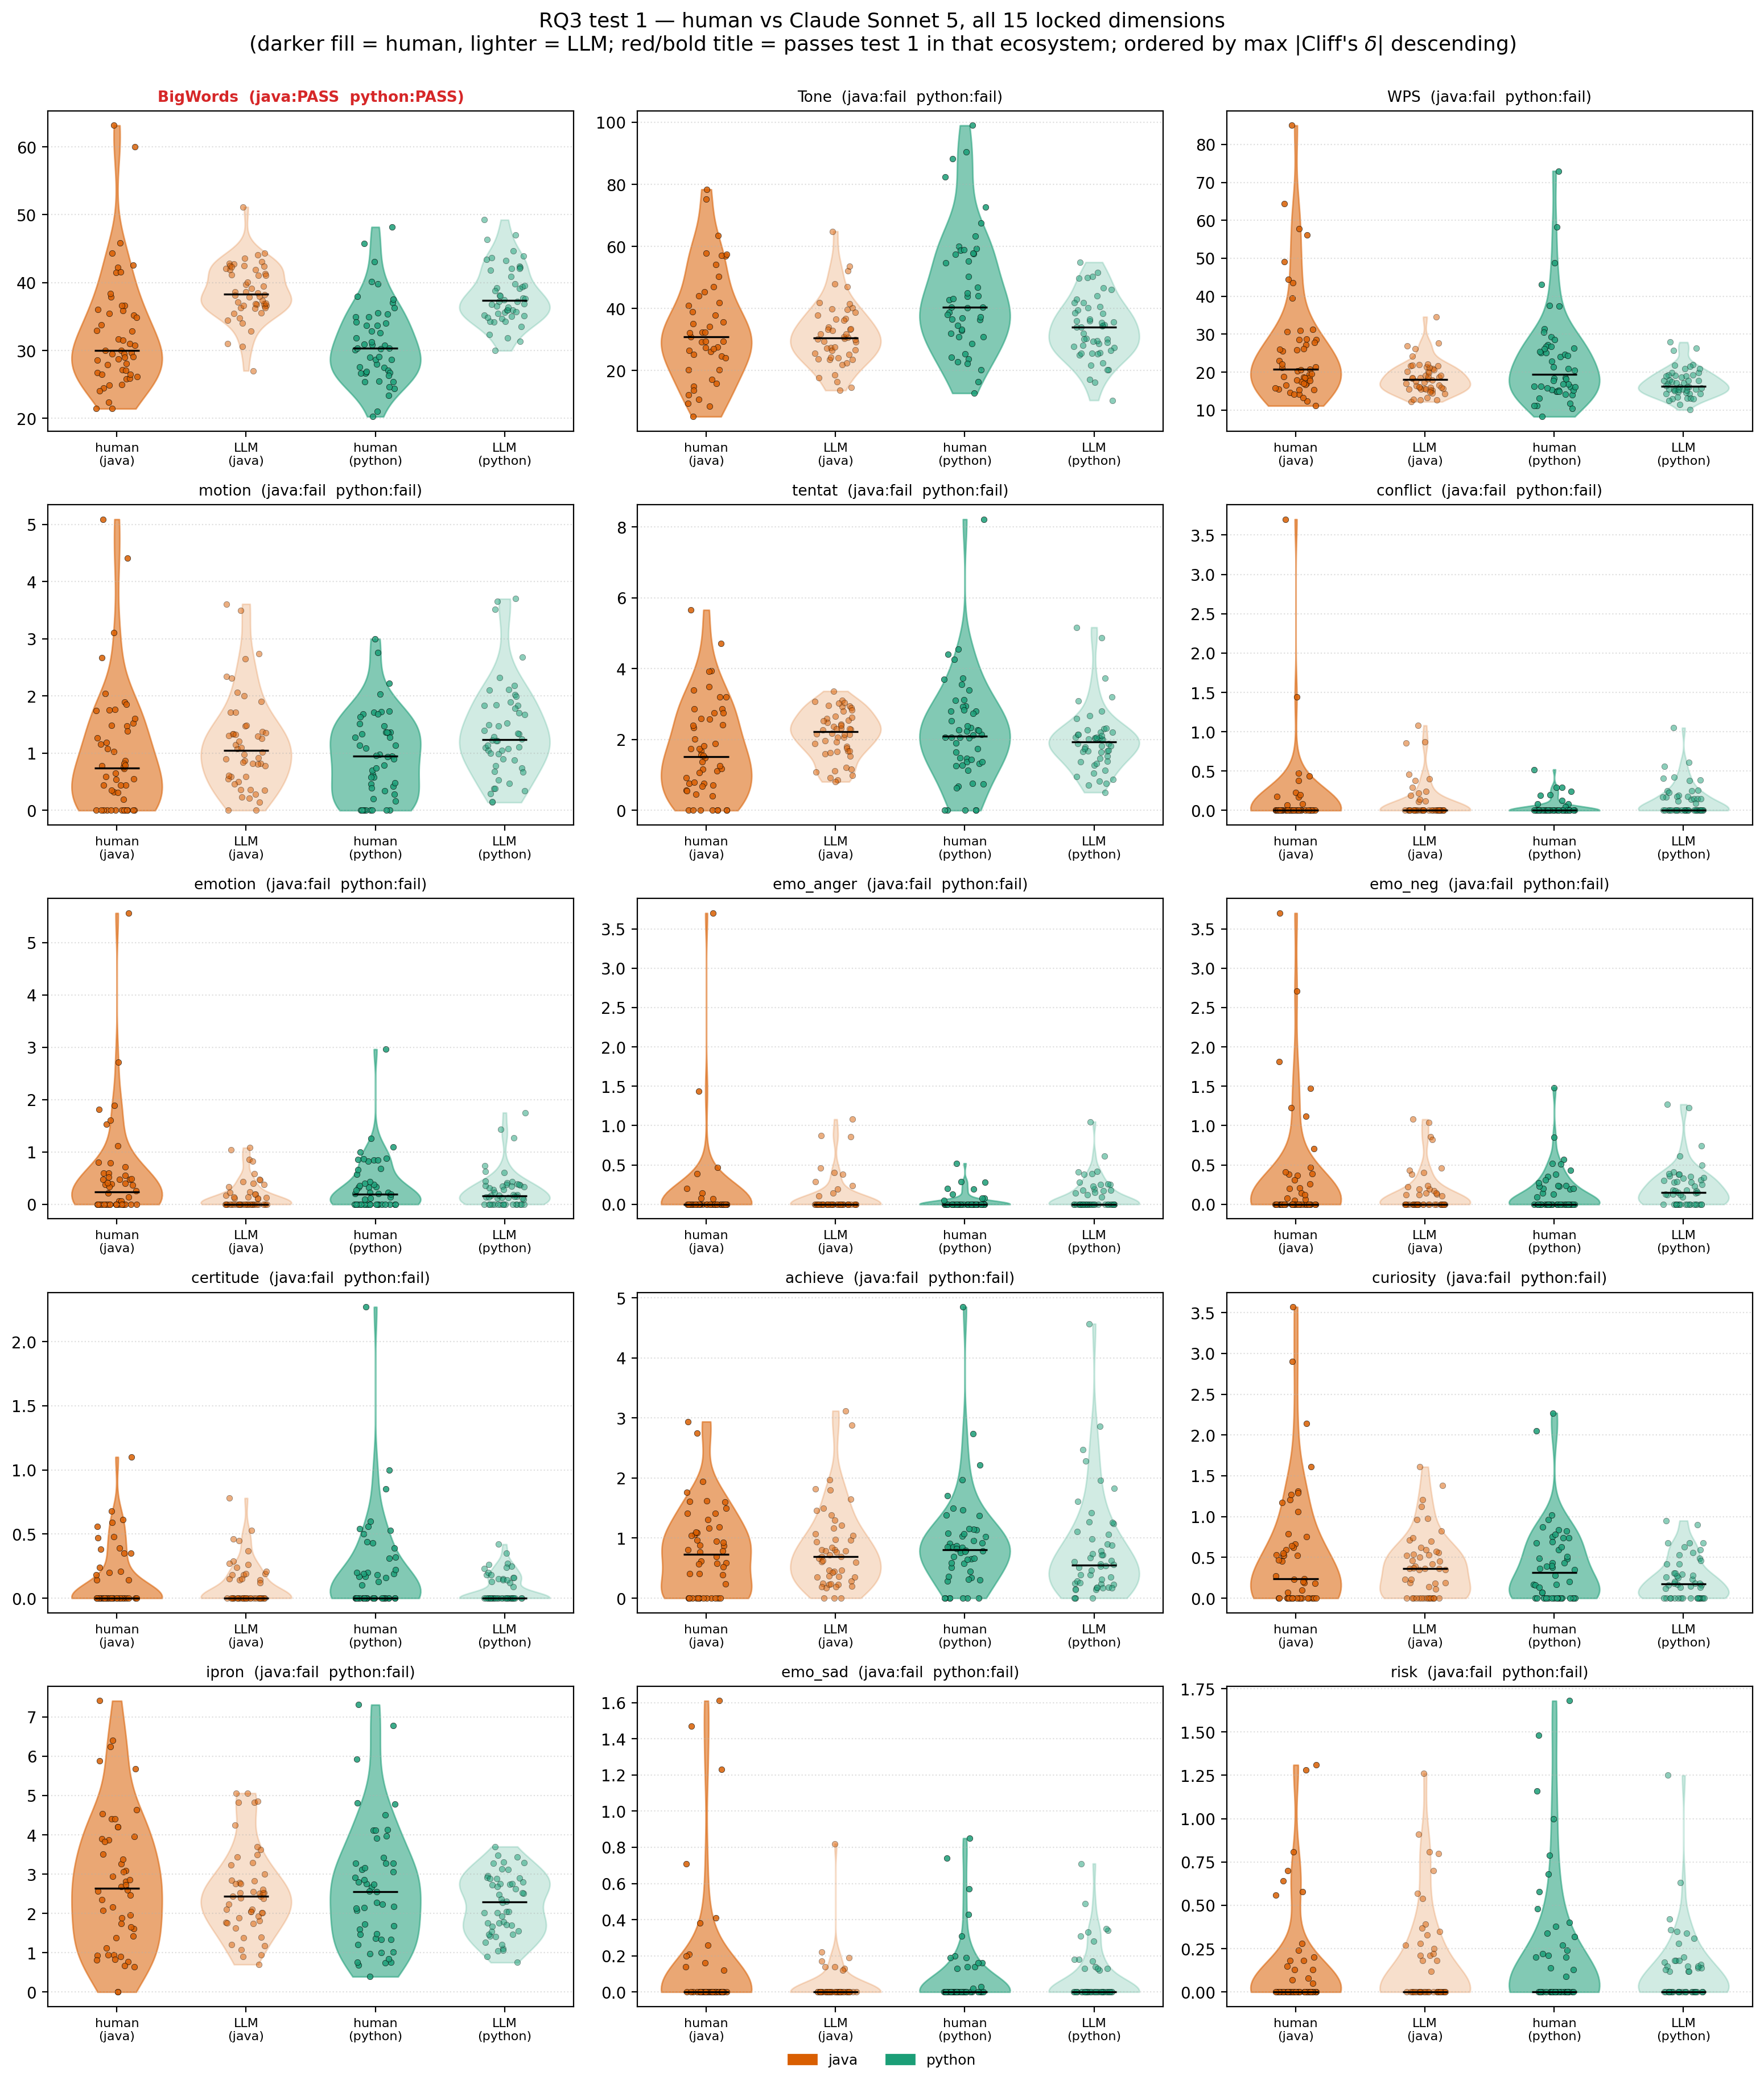
\includegraphics[width=\textwidth]{rq3_02_violin_strip_sonnet.png}}
\caption{RQ3, all 15 locked dimensions: human versus Claude Sonnet~5, per
ecosystem. Darker fill is human, lighter is the model; red titles mark
dimensions clearing test~1 in that ecosystem.}
\label{fig:violin-sonnet}
\end{figure*}

\begin{figure*}[htbp]
\centerline{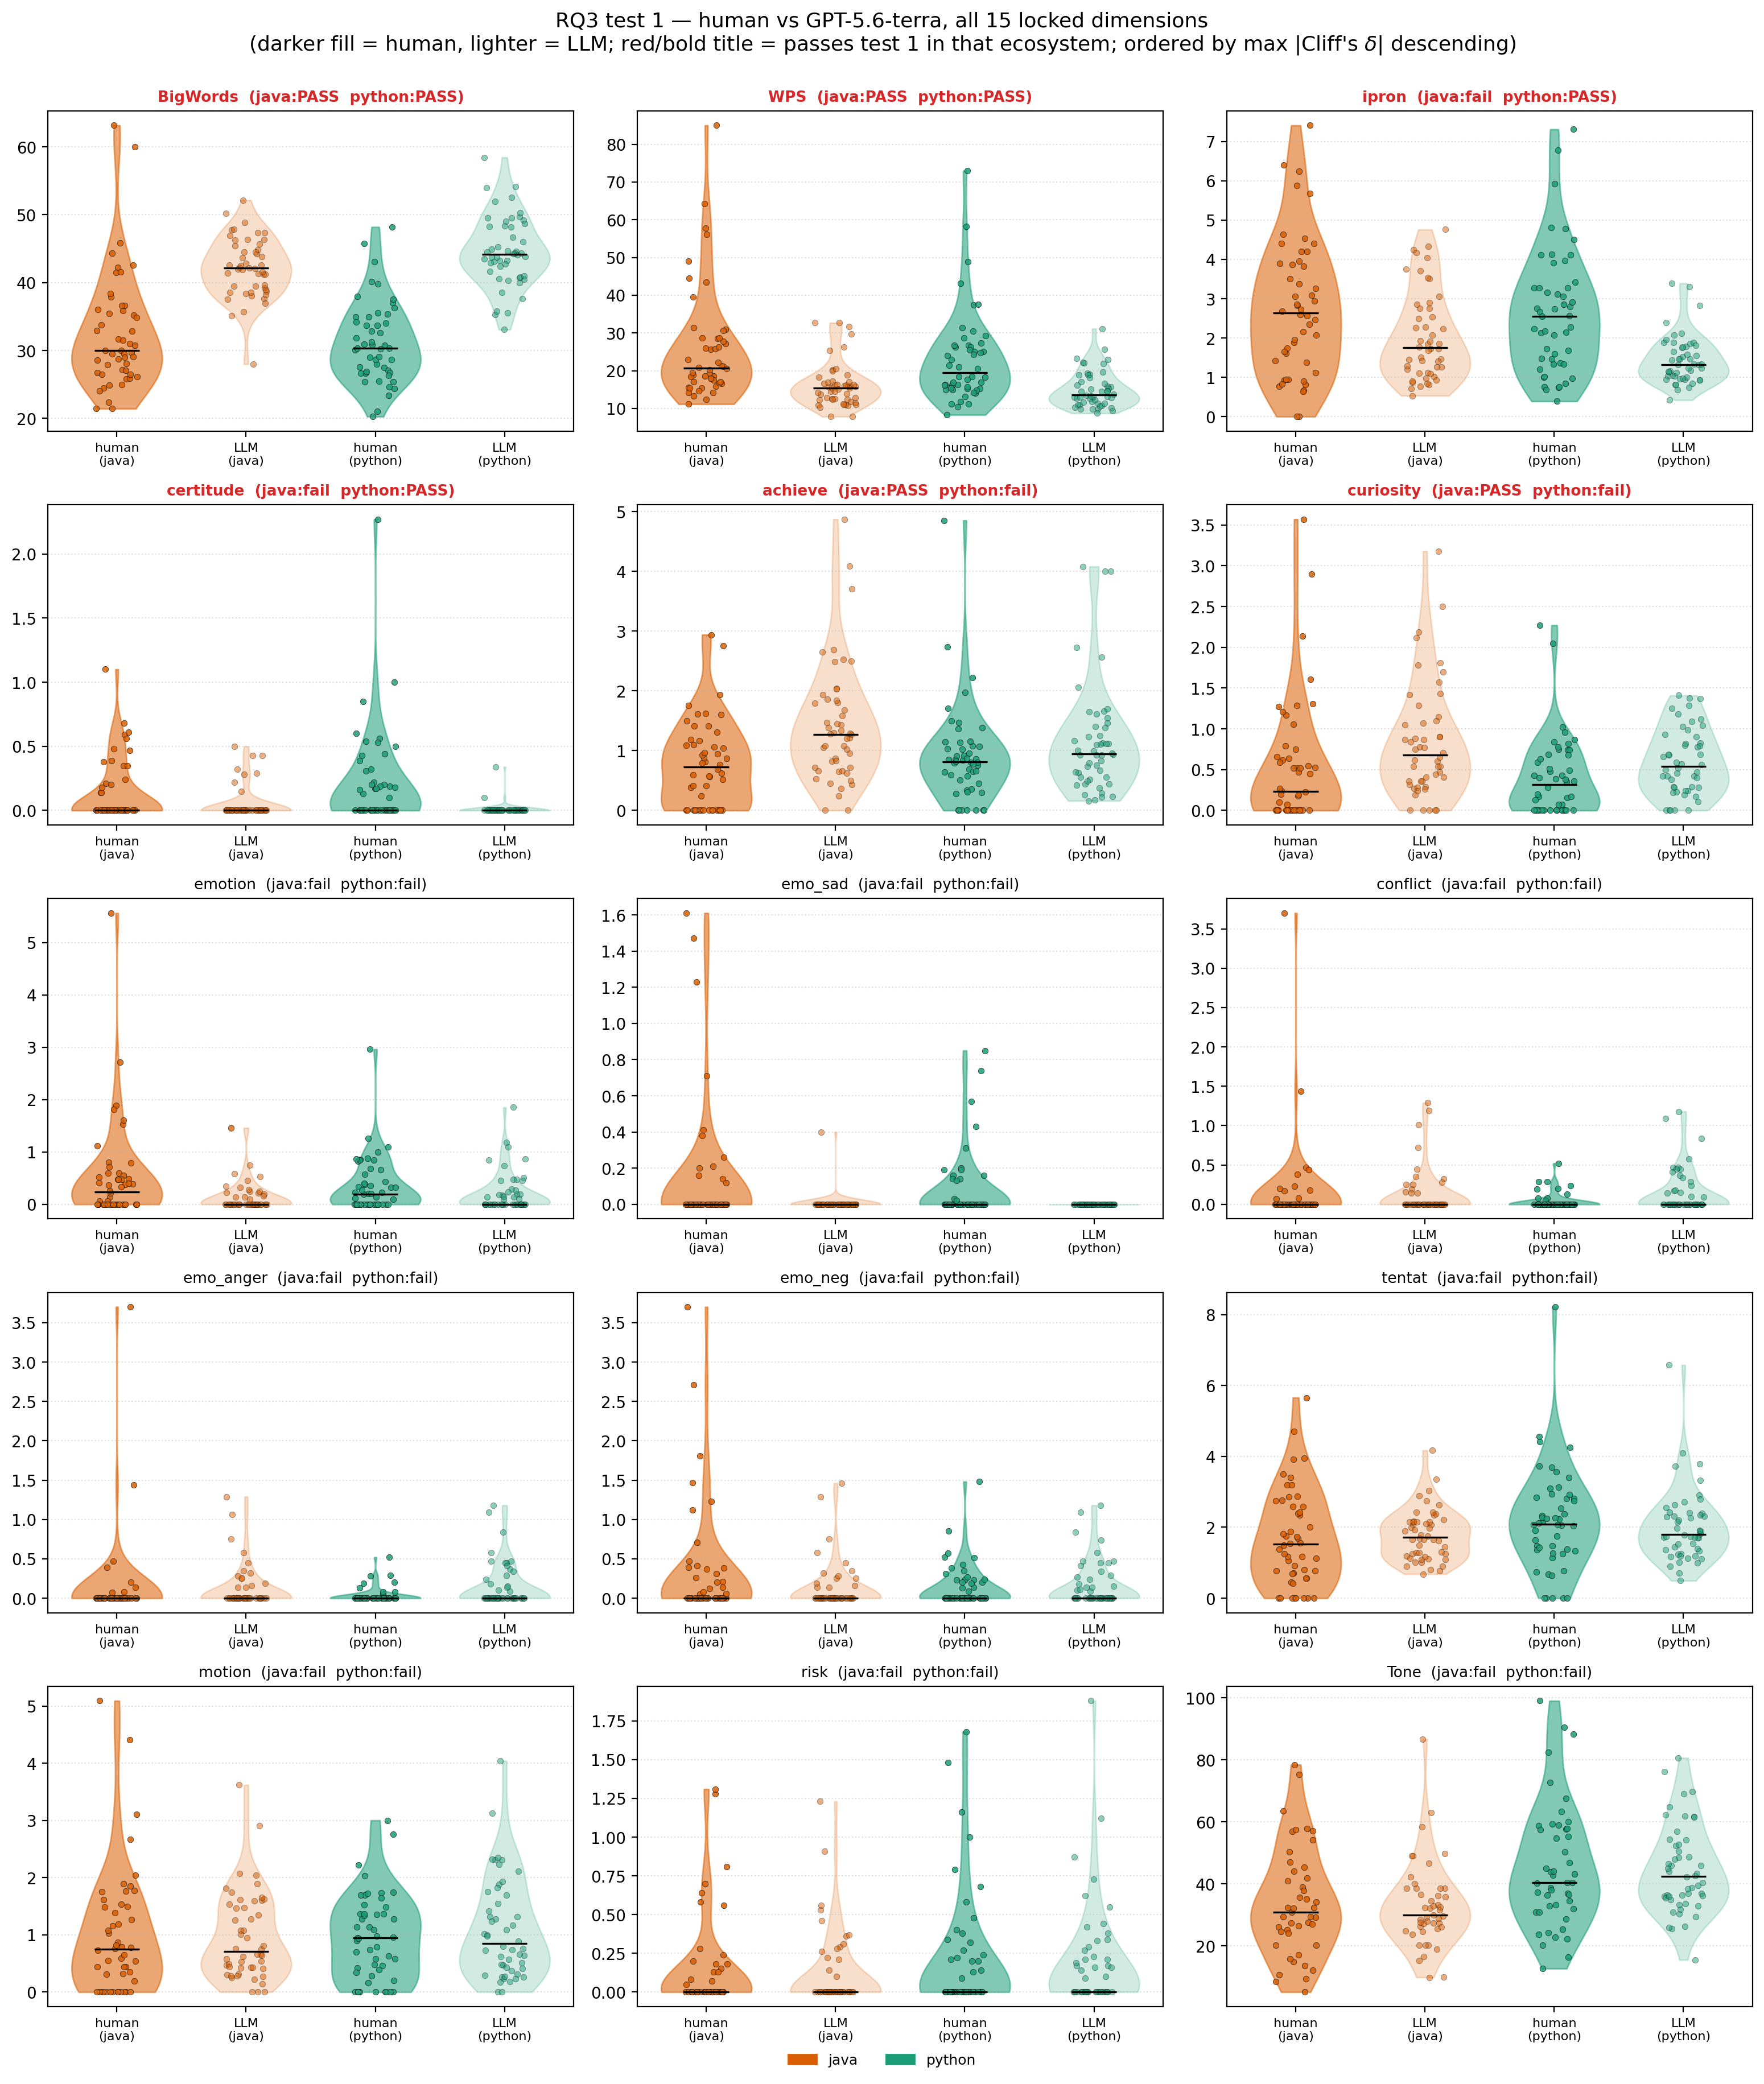
\includegraphics[width=\textwidth]{rq3_02_violin_strip_openai.png}}
\caption{RQ3, all 15 locked dimensions: human versus GPT-5.6-terra, per
ecosystem. Conventions as in Fig.~\ref{fig:violin-sonnet}.}
\label{fig:violin-openai}
\end{figure*}

\begin{figure}[htbp]
\centerline{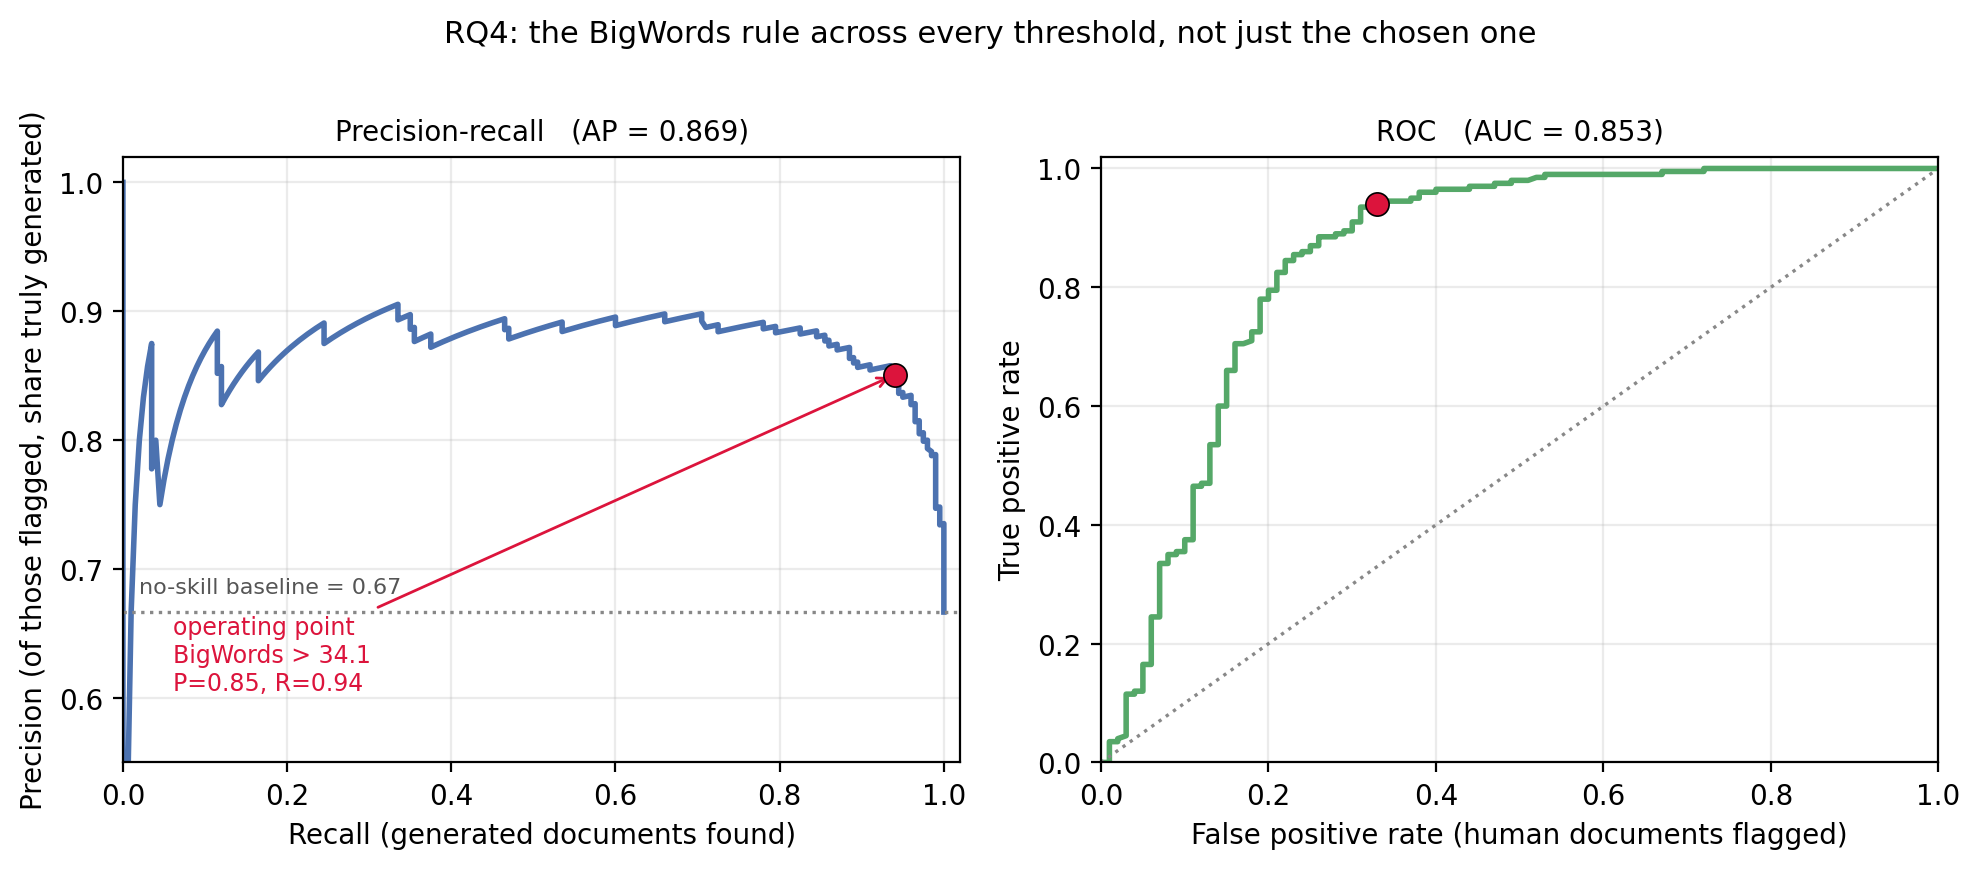
\includegraphics[width=\columnwidth]{rq4_pr_roc.png}}
\caption{RQ4 authorship rule across all thresholds. Left: precision against
recall, no-skill baseline at the positive-class rate ($0.667$), operating point
marked. Right: ROC with the chance diagonal. Average precision and AUC depend
only on the ranking the feature induces, not on any chosen cut-point.}
\label{fig:rq4pr}
\end{figure}

Average precision is $0.869$ against a no-skill baseline of $0.667$, and ROC AUC
is $0.853$ against $0.500$. This means, given one human and one generated document drawn at
random, \texttt{BigWords} orders them correctly 85\% of the time. The shape of
the precision-recall curve also locates the operating point. 

\begin{figure}[htbp]
\centerline{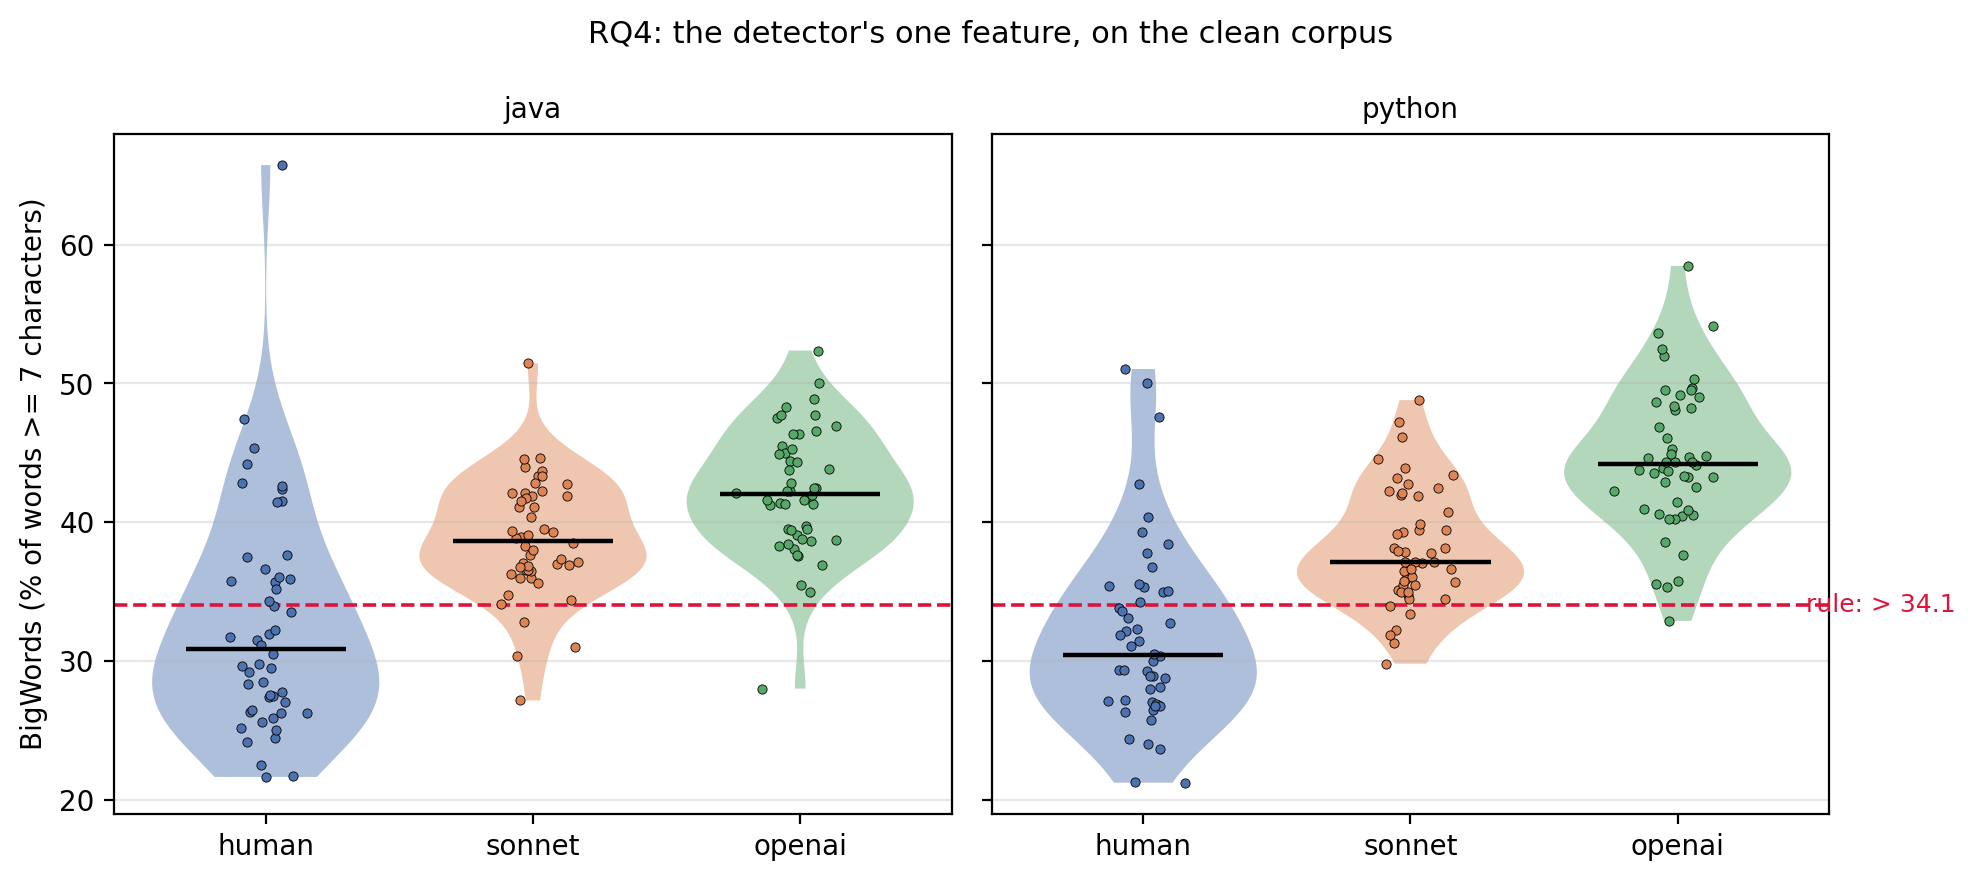
\includegraphics[width=\columnwidth]{rq4_clean_01_bigwords.png}}
\caption{RQ4 detector feature (\texttt{BigWords} recomputed from raw text) for
human, Claude Sonnet~5 and GPT-5.6-terra READMEs, per ecosystem. The dashed
line is the decision threshold (34.1); points on its wrong side are the
detector's errors.}
\label{fig:rq4bw}
\end{figure}

\end{document}
